\documentclass[runningheads]{lib/llncs}
% \documentclass[runningheads,a4paper]{lib/llncs}
\usepackage[english]{babel}
\usepackage[utf8]{inputenc}
\usepackage{xspace}
% \usepackage{cite}
\usepackage{amsmath,amssymb,amsfonts}
\usepackage[noalgohanging,lined,noend,linesnumbered]{algorithm2e}
\SetAlCapSkip{1.5ex}
% \SetAlFnt{\tiny }
% \SetAlFnt{\scriptsize }
\SetAlFnt{\small }
\setlength{\algomargin}{0em}
\SetInd{.1em}{.5em}
% \usepackage{multicol} % does not like llncs
\usepackage[inline]{enumitem}
\usepackage{textcomp}
\usepackage{graphicx,tabularx,placeins}
\usepackage{xcolor}
\usepackage{soul}
% \def\BibTeX{{\rm B\kern-.05em{\sc i\kern-.025em b}\kern-.08em
%     T\kern-.1667em\lower.7ex\hbox{E}\kern-.125emX}}
\PassOptionsToPackage{hyphens}{url}\usepackage{hyperref}
\hypersetup{colorlinks=true, allcolors=black}
\usepackage{subcaption}
\usepackage{mdframed}
%\usepackage[colorinlistoftodos,prependcaption,textsize=tiny]{todonotes}
\usepackage[colorinlistoftodos,prependcaption]{todonotes}
\newcounter{todocounter}
\newcommand{\toreview}{}
\newcommand{\reffig}[1]{Figure \ref{fig:#1}\xspace}

\ifx\toreview\undefined
  \newcommandx{\nota}[2][1=]{}
  \newcommand{\hl}[1]{}

  \newcommandx{\notahl}[2][1=]{}
  \newcommand{\hlhl}[1]{}
  \newcommandx{\notake}[2][1=]{}
  \newcommand{\hlke}[1]{}
  \newcommandx{\notafa}[2][1=]{}
  \newcommand{\hlfa}[1]{}
\else
  % \newcommandx{\nota}[2][1=]{
  %   \stepcounter{todocounter}
  %   \todo[linecolor=red,backgroundcolor=red!25,bordercolor=red,#1]{[\thetodocounter] #2}}
%   \newcommand{\hl}[1]{\colorbox{red!25}{#1}}
  % 
  \newenvironment{highlight}{\begin{mdframed}[backgroundcolor=red!25]}{\end{mdframed}}
  % \newenvironment{myHeartEnv}
  % {\color{purple}{\heartsuit}\kern-2.5pt\color{green}{\heartsuit}}
  % {\text{ forever}}

  % \newcommandx{\notahl}[2][1=]{\stepcounter{todocounter}\todo[
  %   linecolor=green,
  %   backgroundcolor=green!25,
  %   bordercolor=green,#1]{[Helio \thetodocounter] #2}}
  % \newcommand{\hlhl}[1]{\colorbox{green}{#1}}

  % \usepackage{cancel}
  % \newcommandx{\notake}[2][1=]{\stepcounter{todocounter}\todo[
  %   linecolor=yellow,
  %   backgroundcolor=yellow!25,
  %   bordercolor=yellow,#1]{[Kelton \thetodocounter] #2}}
  % \newcommand{\hlke}[1]{\colorbox{yellow}{#1}}

  % \newcommandx{\notafa}[2][1=]{\stepcounter{todocounter}\todo[
  %   linecolor=blue,
  %   backgroundcolor=blue!25,
  %   bordercolor=blue,#1]{[Faria \thetodocounter] #2}}
  % \newcommand{\hlfa}[1]{\colorbox{blue!30}{#1}}

  % \usepackage[showframe,layoutvoffset=0mm,includeall,tmargin=15mm,bmargin=20mm]{geometry}
  % \marginparwidth=34mm
  % \hoffset=-25mm
  % \textwidth=165mm
\fi


\SetAlFnt{\small }
\setlength{\algomargin}{1em}

\makeatletter
\if@twocolumn
\newcommand{\whencolumns}[2]{
#2
}
\else
\newcommand{\whencolumns}[2]{
#1
}
\fi
\makeatother

\begin{document}

\title{
Distributed novelty detection at the edge for IoT network security
\thanks{Thanks to CNPq and  FAPESP for the support.}}
\titlerunning{Distributed ND at the edge for IoT network security}

\author{
  Luís Puhl\inst{1} \and
  Guilherme Weigert Cassales\inst{1}\orcidID{0000-0003-4029-2047}  \and
  Helio Crestana Guardia\inst{1}\orcidID{0000-0001-5010-747X}
  \and
  Hermes Senger\inst{1}\orcidID{0000-0003-1273-9809}
}
\authorrunning{L. Puhl et al.}
\institute{
  Universidade Federal de São Carlos, Brasil\\
  \url{https://www2.ufscar.br/}
}

\maketitle

\newcommand{\refminas}{\textit{Ref}\xspace}
\newcommand{\mfog}{\textit{MFOG}\xspace}
\newcommand{\iot}{IoT\xspace}
\newcommand{\arch}{IDSA-IoT\xspace}
\newcommand{\nids}{NIDS\xspace}
\newcommand{\nd}{DSND\xspace}
\newcommand{\minas}{MINAS\xspace}

\begin{abstract}
% cenário, problema, 
  The ongoing implementation of the Internet of Things (\iot) is sharply
  increasing the number and variety of small devices on edge networks and,
%   break to 2-3 lines
  following this increase, the attack opportunities for hostile agents also
  increases, requiring more from network administrators and the need for tools
  to detect and react to those threats.
  % 
  One such tool are the Network Intrusion Detection Systems (\nids)
  which captures and analyses network traffic,
  acting when a known attack or a new pattern is detected.
  For a network security tool to operate in the context of edge and
  \iot it has to comply with processing, storage and energy
  requirements alongside traditional requirements for stream and network
  analysis like accuracy and scalability.
  % 
  Using a previously defined architecture (\arch),
  we address the construction and evaluation of a distributed \nids
  with the Data Stream Novelty Detection (\nd) algorithm MINAS
  employing C and MPI library.
%   apresentar a estratégia,
  % 
  We discuss the algorithm steps, how it can be deployed in a distributed
  environment, the impacts on the accuracy and evaluate performance and
  scalability using a cluster of constrained devices commonly found in \iot
  scenarios.
  % 
  % We found an increase of \textit{A 0.0} processed network flow descriptors per
  % core added to the cluster.
  % Also \textit{B 0.0\%} and \textit{C 0.0\%} change in
  % \textit{F1Score} in the tested datasets when stream was unlimited in speed and
  % limited to \textit{0.0 z MB/s} respectively.
  We found a marginal ($2$ to $4\%$) difference in true positive (hits) between
  original, serial and distributed executions, consuming a months worth of flow
  descriptors in $300$ seconds.
%   concluindo que é viável e barato utiliar este tipo de abordagem
  \todo[inline]{Manter IDS? Fazer novelty detection distribuído utilizando recursos na borda, em pequenos dispositivos buscado escalabilidade (?) e baixa latência, 
  Os resultados mostram que ..., permitindo concluir que ... }
\end{abstract}

\ifdefined\IEEEkeywords
\begin{IEEEkeywords}
  % Detecção de Novidades, Detecção de Intrusão, Fluxos de Dados, Computação Distribuı́da, Computação em Névoa, Internet das Coisas.
  novelty detection, intrusion detection, data streams,
  distributed system, edge computing, internet of things
\end{IEEEkeywords}
\else
\keywords{
novelty detection \and intrusion detection \and data streams \and
distributed system \and edge computing \and internet of things
}
\fi


% \listoftodos
% \todototoc

\section{Introduction}


% \todo{poderia trocar esses surveys por mais novos ou menos preditivos e mais acertvivos}

% A survey released by Gartner estimated about 20 billion devices connected to the
% Internet by 2020, many of them through the IoT \cite{gartner_forecast_2017}.
% More recently, Statista predicted that the total number of such devices will
% reach 38 billion by 2025, and 50 billion by 2030 \cite{statista-iot}.
The Internet of Things (\iot) brings together a wide variety of devices,
including mobile, wearable, consumer electronics, automotive and sensors of
various types.
% 
Such devices can either be accessed by users through the Internet or connect
to other devices, servers and applications,
with little human intervention or supervision
\cite{Tahsien2020,abane2019,haddadpajouh2019survey,Shanbhag2015}.
% 
Security and privacy is a major concern in the \iot, especially regarding
% devices like smart home assistants and wearable
devices having access to user personal data like
location, health and many other sensitive data \cite{sengupta2020comprehensive}.
% 
Furthermore, if compromised, such devices can also be used to attack other
devices and systems, steal information, cause immediate physical damage or
perform various other malicious acts \cite{Kolias2017mirai}.
% 
As an additional concern, \iot devices likely have a long lifespan, less frequent
software patches, growing diversity of technologies combined with lack of
control over the software and hardware of such devices by the host organization
(where they are deployed), which considerably increases the attack surface.

% A study reveals that nearly $20\%$ of organizations have experienced at least one
% IoT-based attack in the last three years.
% The study shows that most organizations have no control over the origin and
% nature of software and hardware used by the connected devices.
% To protect against these threats, the IoT industry's spending on security is
% estimated to be around USD $\$\,3.1$ billion in 2021 \cite{gartner_it_glossary_2018}, 
% which includes the development of tools
% and services to improve asset discovery and management, software security
% evaluation, hardware % testing 
% and penetration testing.

% i.e. 'id est', which means "that is."
% e.g. 'exempli gratia', which means "for example."
% {\color{red} muito próximo de \cite{Cassales2019a}}
Because most \iot devices have limited resources (i.e., battery, processing,
memory and bandwidth), configurable and expensive algorithm-based
security techniques are not usual, giving way to network based approaches 
% may not fit 
\cite{Zhou2017}.
Machine Learning (ML) techniques, for instance, have been studied for years to detect attacks
from known patterns or to discover new attacks at an early stage
\cite{buczak2016survey,mitchell2014survey}.
A recent survey \cite{Tahsien2020} shows that ML based methods are a
promising alternative which can provide potential security tools for the \iot
network making them more reliable and accessible than before.

Despite the promising use of ML to secure \iot systems, studies found in the
literature \cite{buczak2016survey,mitchell2014survey,Tahsien2020} are limited to
traditional ML methods that use static models of traffic behavior.
% With traditional ML methods, the data set is static and can be traversed
% repeatedly, and the detection of new attack patterns requires a new cycle of
% training, testing, and dissemination of new models.
Most existing ML solutions for network-based intrusion detection cannot maintain
their reliability over time when facing evolving attacks \cite{Viegas2019,AndreoniLopez2019}.
Unlike traditional methods, stream mining algorithms can be applied to intrusion
detection with several advantages, such as:
\begin{enumerate*}[label=(\emph{\roman*})]
    \item processing traffic data with a single read;
    \item working with limited memory (allowing the implementation in small
    devices commonly employed in edge services);
    \item producing real-time response; and
    \item detecting novelty and changes in concepts already learned.
\end{enumerate*}

% Nao tinha mencionado quais previous works...
% {\color{red} %This paper elaborates on the previous work in the following aspects.

% {\color{red} Adicionar referencias e relacionados. Argumentar que além de \nids,
% \nd para \iot tem outras aplicações}

% CATRACA \cite{AndreoniLopez2018,AndreoniLopez2019} SBRC AndreoniLopez2019
% BigFlow \cite{Viegas2019}
Given the recent \cite{Viegas2019,AndreoniLopez2019,DaCosta2019a} use of Data Stream Novelty
Detection (\nd) in network data streams, this paper shows the effects of
adapting these mechanisms to edge services for use in \iot environments.
Our proposal, called \mfog, adapted the \arch
architecture \cite{Cassales2019a} using the \nd algorithm \minas
\cite{Faria2013Minas,Faria2016minas}, making it suitable to run
% (as it was already tested in a similar \iot scenario) 
on a distributed system composed of small devices with limited
resources on the edge of the network.
% Our implementation can be fully executed on the edge, thus avoiding any dependency
% and high latency of cloud resources.
% We proposed and implemented dMINAS, a distributed extension
% of MINAS \cite{Faria2016minas} (a novelty detection for data streams).
Using our newer version of the \minas algorithm, we have experimentally evaluated 
% through experimental methodology, 
how the distribution 
% the chosen novelty detection algorithm \minas
affects the capability to detect changes (novelty) in
traffic patterns and its impact on the computational efficiency.
Finally, some distribution strategies and policies for the data stream
novelty detection system are discussed.
% }

% \begin{figure}[hb]
%     \centering
%     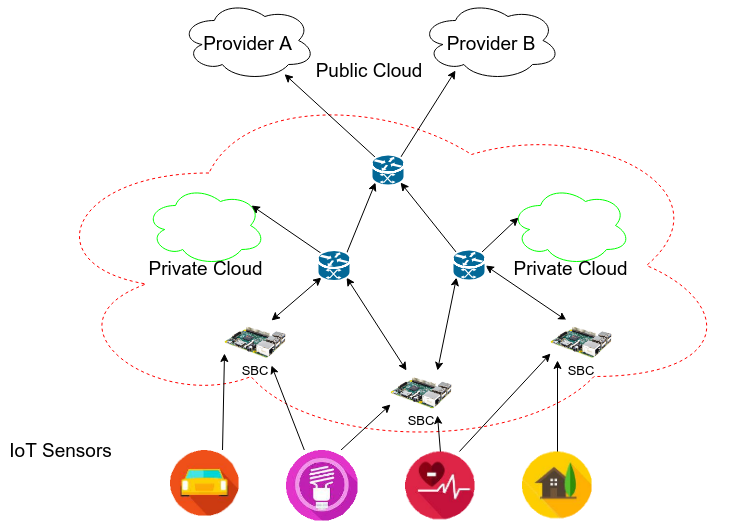
\includegraphics[width=0.5\linewidth]{figures/cassalesimgs-000.png}
%     \caption{\arch \cite{Cassales2019a} physical architecture and deployment scenario overview.}
%     \label{fig:mfog-phy-arch-cloud}
% \end{figure}

This paper is organized as follows:
% Section \ref{sec:related} presents the related works.
Section \ref{sec:minas} reviews the chosen \nd algorithm \minas.
A distributed extension of \minas, including its
implementation and evaluation are presented in Section \ref{sec:prop}
and in Section \ref{sec:experiments} we show how we evaluated \mfog and
the discuss results we found.
Finally, Section \ref{sec:conclusion} summarizes the main findings and presents
possible future work.

% \todo{Parei aqui a redação da Introdução.Deixei grifado em vermelho o
% paragrafo que fala das contribuições. Talvez com um pequeno esforço em
% especificar uma versão distribuida do MINAS teriamos uma extensão do mesmo. }

% Desafios de arquitetura e validação:

% - Construção de um protótipo da arquitetura IDSA-IoT:
%   - Kafka (Python): Distribuição e balanceamento pelo cluster kafka, hipótese refutada.
%   - Flink (Java ou Scala): Execução do cluster nos dispositivos de névoa, hipótese refutada.
%   - MPI (C e Python): Execução do cluster nos dispositivos de névoa, hipótese aceita.
% - Reimplementação do algoritmo MINAS com fidelidade:
%   - Duas versões: a descrita e a implementação de referência (em Java).
%   - Resolução: utilizar a descrição, não *seguir* a imp. referência, apenas como ponto de comparação. Exemplos:
%     - Definição de raio `r = f * σ` (fator vezes desvio padrão) para `r = max(distance)` (distância máxima);
%     - Tamanho do buffer de desconhecidos e frequência de execução do passo de detecção de novidade;

% \begin{highlight}
% Expected results:
% A system that embraces and explores the inherent distribution of fog computing
% in a IoT scenario opposing regular systems where data streams are collected and
% centralized before processing;
% Impact assessment of the impact of distributed, regional flow characteristics,
% local vs global vs distributed forgetting mechanism and other policies.

% IDS characteristics and description of physical scenario.

% MINAS characteristics.

% Distribution and IDSA-IoT architecture.
% \end{highlight}

% This paper is structured as follows:
% Section \ref{sec:related} presents previous works that addresses related
% problems and how they influenced our solution.
% Section \ref{sec:implementation} address our proposal, the work done, issues
% found during implementation and discusses parameters and configurations options
% and how we arrived at our choices.
% Section \ref{sec:experiments} shows experiments layouts and results, we
% compare serial and distributed implementation's metrics for validation,
% we also evaluate communication delay effects on classification metrics and
% conclude with the speedup per core and overall maximum stream speed.
% Section \ref{sec:conclusion} summarizes the research results and presents our
% final conclusions and future works.
%\FloatBarrier
% 
% ----------------------------------------------------------------------------------------------------------------------
\section{Related Work}
\label{sec:related}

Network Intrusion Detection based on Machine Learning is not a novel concept.
The plethora of network applications and 
ways of exploiting them, motivate using automated means to detect known and novel attacks. 
% the interest of teach a machine how to detect a novel attack is formed.
There are, though, open questions and challenges on this subject, such as
reducing false positive rate and detecting attacks in a timely fashion \cite{DaCosta2019a}.

A few recent works inspired our work, such as: BigFlow \cite{Viegas2019}
employing Apache Kafka and Apache Flink for distributed stream processing,
four algorithms (Hoeffding Tree, OzaBoosting, Leveraging Bag) and one Ensemble
from the Massive Online Analysis (MOA) library \cite{MOA}, and
evaluating with package stream dataset solving the time constraint for \nids;
CATRACA \cite{Lopez2018,AndreoniLopez2019a}, in a similar way, uses 
Apache Kafka and Apache Spark for stream processing and also achieves
a timely and scalable \nids.

% % {\color{red} muito próximo de \cite{Cassales2019a}}
% 6LoWPAN is a standard defined by the IETF in RFC 6282, to transmit data with
% IpV6 and other protocols on low power wireless devices using IEEE 802.15.4 in
% the lower layers. However, this technology still lacks protection and security
% mechanisms. %\cite{dos-6lowpan-iot, Hybrid-ids-arch-iot, SVELTE}.
% %
% For instance, in \cite{dos-6lowpan-iot}, signature detection is used to detect
% DoS and UDP flood attacks. The architecture uses a probe to promiscuously listen
% the whole traffic of a 6LoWPAN network and sends the data to analysis on a
% non-constrained host.
% %Results were expressed by flood metrics, as the number of packets in the network.
% The work in \cite{SVELTE} proposed an hybrid IDS which focuses on specific
% routing attacks, such as sink-hole and selective-forwarding. Higher complexity
% tasks which demand more computational resources are executed on the border
% router, while simpler tasks execute on constrained nodes. Results were expressed
% by metrics as recall and memory and energy consumption.
% % 
% The work in \cite{Hybrid-ids-arch-iot} proposed the use of anomaly detection to
% identify internal routing attacks, and signature detection to identify external
% attacks. Anomaly detection was tested with simulated attacks, while signature
% detection used a subset of NSL-KDD. They used the recall and FAR as metrics.

A three-layer architecture (composed of WSN, Fog and Cloud) with focus on fault
tolerance in disaster scenarios is proposed in \cite{Fault-tolerance-disaster}.
Fog computing is used to execute ML functions and data aggregation. Experiments
used real data collected from sensors. The metrics used included precision,
recall and accuracy.
%
The work in \cite{Kalis} proposed an hybrid IDS which collects information about
the environment and activates specific modules to mitigate each kind of attack.
Experiments were made in a real environment and metrics used were recall,
precision and resource consumption (CPU and RAM).
%
Smart cities scenarios also employ IoT to measuring and monitoring tasks.
%\cite{IoT-arch-smartmeter,scalable-anomaly-detection-smart-city,DS-based-IDS-SmartGrid}.
In \cite{IoT-arch-smartmeter}, the authors propose an architecture that uses
three stream mining methods based on ML to characterize water and energy
consumption behavior, predict consumption, and detect incidents.
The metrics used to express results include water and energy consumption.
%
The work in \cite{scalable-anomaly-detection-smart-city} also aimed to identify
anomalies in a water distribution network and proposes a three layer
architecture (sensors, base stations and datacenter).
The second layer performs time-sensitive tasks, thus reducing latency, while
third layer provides storage and aggregates the results of the second layer with
historical data to generate more accurate information.
Water distribution measures were used, comparing the values of the predictions
with the actual measurements.
%
Intrusion detection for smart cities, based on data mining techniques running on
an unrestricted devices is proposed in \cite{DS-based-IDS-SmartGrid}.
Experiments using KDD99 data are presented and the metrics used were precision,
Kappa, memory consumption, time, FAR, and FNR.


Table \ref{tab:summary} summarizes the discussion on the related work.
Note that some works use data from KDD99 or derived from this dataset.
Collected two decades ago, KDD is no longer representative of current attack
patterns and IoT environments.
Some works used traces captured from local infrastructure, which provide
realistic evaluation, but lack of reproducibility.
Some works used data produced by intentional simulated attacks, designed by the
same people who designed the detection techniques.
This can bring unrealistic advantages to the detection methods.
Also, it is worth noting that most articles used metrics like FAR, recall, and
accuracy.
Although widely adopted in classical scenarios, such metrics are inaccurate for
stream processing \cite{GAMA2010}.

\begin{table*}[htb]
\caption{Summary of related works}
\centering
\begin{scriptsize}
% \begin{tabularx}{\textwidth}{ l m{2cm} | m{2cm} l m{2cm} | m{2cm} | m{2cm} | m{2cm} }
\begin{tabularx}{\textwidth}{l|l|X|X|X}
% \begin{tabularx}{\textwidth}{l|l|X|X|m{3.0cm}}
% Trabalho & Platforma  & Técnica & DataSet & Métricas \\
Work                                         & Platforms    & Technique & DataSet & Metrics\\\hline\hline
% Kasinathan et al
\cite{dos-6lowpan-iot}                       & 6LoWPAN      & Suricata & Real data with metasploit & Accuracy, packets/second\\\hline
% Sheikhan and Bostani
\cite{Hybrid-ids-arch-iot}                   & 6LoWPAN      & Hybrid - MR OPF & NSL-KDD and simulated attacks & FAR and recall\\\hline
% Raza et al
\cite{SVELTE}                                & 6LoWPAN      & DAG analysis & No information & Recall, energy and memory consumption\\\hline
% Furquim et al
\cite{Fault-tolerance-disaster}              & WSN          & MLP of Weka & Real data & MAE, RMSE, R², R, accuracy, recall, precision, specificity\\\hline
% Midi et al
\cite{Kalis}                                 & WSN          & Independent modules, each with one technique & Trace replay and attack injection & Recall, accuracy, memory and CPU consumption\\\hline
% Lloret et al
\cite{IoT-arch-smartmeter}                   & Smart City   & Clustering, MLP and statistical models & Real data from meters & Water and energy consumption\\\hline
% Diffalah et al
\cite{scalable-anomaly-detection-smart-city} & Smart City   & LiSA, smoothing function & Real data & Outliers, comparison between simulation and collected data\\\hline
% Faisal et al
\cite{DS-based-IDS-SmartGrid}                & Smart Grid   & 7 MOA classifiers & KDD99 & Accuracy, Kappa, memory consumption, time, FAR and FNR \\\hline
\end{tabularx}
\label{tab:summary}
\end{scriptsize}
\end{table*}

% ----------------------------------------------------------------------------------------------------------------------
% - Escrever! Corpo:
%   - Proposal (retomar problema {iot, sec, ND}, objetivo, soluções {minas, paralelismo, distribuído, ~~py-kafka, flink,~~ mpi}, propor uma solução)
%   - Implementation (mpi, c, data-structures, data-flow, )
%   - Experiments (rpi, cluster, `evaluate.py`)
%   - Results
%   - Conclusion
% - Demonstrar o paralelismo com figura de pipeline (time vs instruction)
%\FloatBarrier
\section{MINAS}
\label{sec:minas}

%  ******************* Texto quali ************************
% \subsection{O Algoritmo MINAS}
% Apresentar o MINAS de forma resumida (1 pagina no max): como funciona, etc. 

MINAS is an offline-online clustering algorithm, which means it has two distinct phases.
The first phase generates the model by creating several micro-clusters based
on a separate training set that is processed offline.
Each micro-cluster can be associated with only one class of the problem,
but each class can have many micro-clusters.
The online phase is where the model performs three tasks in (near) real-time.
% Our proposal focuses on the online phase, therefore we will describe it in more detail.
We describe the online phase in more detail since we focus on its tasks. 

In summary, MINAS executes the classification, novelty detection,
and model update tasks in the online phase.

% ******************* OLD ******************* 
% % classification
% For each arriving instance, the model tries to explain (i.e, classify) the instance by associating it with an existing micro-cluster. 
% % update
% If there is a micro-cluster within a parameterizable distance of the instance, the instance is grouped in that micro-cluster  by adding (i.e., updating) its attributes to the micro-cluster's feature vector. 
% % temp memory + ND
% Otherwise, this instance will be considered unknown and saved on a temporary memory for future use. 
% When the size of the temporary memory reaches a parameterizable value MINAS stops classifying new instances and performs the novelty detection process. 
% The novelty detection tries to find 
% % linha abaixo pode ser omitida se achar melhor
% valid and representative (i.e., \textit{silhouette} > 0 and at least a parameterizable number of instances) 
% groups of unknown instances from the temporary memory.
% Each 
% % linha abaixo pode ser omitida se achar melhor
% % valid and representative
% group found can be a new pattern if the distance between it and its closest micro-cluster is bigger than a parameterizable threshold or, otherwise, an extension of said micro-cluster.
% ******************* NEW ******************* 
MINAS tries to classify each incoming unlabeled instance according to the
current decision model. Instances unexplained by the model
% pode descomentar linha abaixo para dar mais "detalhes"
% (i.e., distance from all existing micro-clusters bigger than a parameterizable threshold)
receive an \textit{unknown} label and are stored in temporary memory for future
analysis.
When this temporary memory reaches a parameterizable size, MINAS groups the
instances to form new micro-clusters.
Each micro-cluster is validated to discard the non-cohesive or unrepresentative
ones.
Valid micro-clusters are analyzed to decide if they represent an extension of a
known pattern or a completely new pattern. In both cases, the model absorbs the
valid micro-clusters and starts using them to classify new instances.
MINAS also has a mechanism to forget micro-clusters that became obsolete and
unrepresentative of the current data stream distribution.
Besides, MINAS also cleans the temporary memory to eliminate ungrouped unknown
instances as they represent noise~\cite{Faria2016minas}.

% Citar que o trabalho anterior já validou o uso do MINAs para detecção de novidade porem com uma implementação sequencial. 

Authors in~\cite{Cassales2019a} validated the usage of the MINAS algorithm for
the Intrusion Detection and deploying it on edge. However, they used the
sequential version of the algorithm, where classification stops completely to
execute novelty detection.

% Figura do MINAS (offline + online) ...
% \todo[inline, color=brown]{\textbf{Guilherme:} Não coloquei figura porque as figuras originais do MINAS ocupam bastante espaço (https://sci-hub.se/10.1007/s10618-015-0433-y pg 9) e a do MFog está mais completa.}

{\color{red}Formally, a data stream $S$ is a massive sequence of data elements
$x_1, x_2, \dots, x_n$ that is, $S={\{x_i\}}_{i=1}^n$, which is potentially
unbounded (n → $\infty$).
Compared to traditional (batch) data mining, stream processing algorithms have
additional requirements.
For instance, with a potentially infinite data stream, storing data for late
processing is not a choice due to memory constraints.
Algorithms need to incrementally process incoming data instances in a single
pass while operating under memory and response time constraints.
Furthermore, as data streams present transient behavior, prediction models often
need to be incremented to adapt to concept drift observed in data. }


% \begin{algorithm}
%     \DontPrintSemicolon
%     \SetKwFunction{FMain}{Main}
%     \SetKwProg{Fn}{algorithm}{:}{}
%     \Fn{\FMain{$f$, $a$, $b$, $\varepsilon$}}{
%           a\;
%           b\;
%           \KwRet\;
%     }
%     \;
%     \SetKwProg{Pn}{algorithm}{:}{\KwRet}
%     \Pn{\FMain{$f$, $a$, $b$, $\varepsilon$}}{
%           a\;
%           b\;
%     }
% \end{algorithm}
% \IncMargin{1em}
\begin{algorithm}[h]

% \begin{multicols}{2}
    \SetKwProg{Function}{Function}{:}{}
    % \DontPrintSemicolon
    % \KwIn{sample, ModelSet, params as p}
    % \KwOut{Classified Sample}
    % 
    \SetKwData{CW}{cleaningWindow}
    \SetKwData{NDT}{noveltyDetectionTrigger}
    \SetKwData{MEPC}{minExamplesPerCluster}
    \SetKwData{NF}{noveltyFactor}
    % 
    % \KwSty{Parameters}: cleaningWindow as \CW,
    % noveltyDetectionTrigger as \NDT,
    % minExamplesPerCluster as \MEPC,
    % noveltyFactor as \NF\\
    % 
    \SetKwFunction{nearestCluster}{nearestCluster}
    \SetKwFunction{clustering}{clustering}
    \SetKwFunction{sizeOf}{sizeOf}
    \SetKwFunction{NoveltyDetection}{NoveltyDetection}
    \SetKwFunction{handleModelSleep}{moveToSleep}
    \SetKwFunction{removeOldSamples}{removeOldSamples}
    % 
    % \KwData{ UnkownSet $\leftarrow$ $\emptyset$, ModelSleepSet $\leftarrow$ $\emptyset$, lastCleanupTime $\leftarrow$ now() }
    % 
    \Function{\NoveltyDetection{Model, Samples}}{
        newModelSet $\leftarrow$ $\emptyset$\;
        \ForEach{cl in \clustering(Samples)}{
            \If{$|cl.sampleSet| \geq$ \MEPC}{
                (distance, near) $\leftarrow$ \nearestCluster(cl, Model)\;
                \eIf{distance $<$ near.radius $\times$ \NF}{
                    cl.label $\leftarrow$ near.label\;
                    cl.type $\leftarrow$ extension\;
                }{
                    cl.label $\leftarrow$ noveltyIndex\;
                    noveltyIndex $\leftarrow$ noveltyIndex $+ 1$\;
                    cl.type $\leftarrow$ novelty\;
                }
                Samples $\leftarrow$ Samples $\ominus$ cl.sampleSet\;
                newModelSet $\leftarrow$ newModelSet $\oplus$ cl\;
            }
        }
        \Return{newModelSet}
    }
    \label{alg:MINAS-nd}
    \caption{Minas: Novelty Detection task.}
\end{algorithm}
\begin{algorithm}
    \SetKwProg{function}{Function}{:}{}
    % \DontPrintSemicolon
    % \KwIn{sample, ModelSet, params as p}
    % \KwOut{Classified Sample}
    % 
    \SetKwData{CW}{cleaningWindow}
    \SetKwData{NDT}{noveltyDetectionTrigger}
    \SetKwData{MEPC}{minExamplesPerCluster}
    \SetKwData{NF}{noveltyFactor}
    % 
    % \KwSty{Parameters}: cleaningWindow as \CW,
    % noveltyDetectionTrigger as \NDT,
    % minExamplesPerCluster as \MEPC,
    % noveltyFactor as \NF\\
    % 
    \SetKwFunction{nearestCluster}{nearestCluster}
    \SetKwFunction{clustering}{clustering}
    \SetKwFunction{sizeOf}{sizeOf}
    \SetKwFunction{NoveltyDetection}{NoveltyDetection}
    \SetKwFunction{handleModelSleep}{moveToSleep}
    \SetKwFunction{removeOldSamples}{removeOldSamples}
    % 
    \SetKwProg{algorithm}{algorithm}{:}{}
    \SetKwFor{With}{with}{}{}
    \SetKw{continue}{continue}
    % 
    \SetKwData{CW}{CW}
    \SetKwData{noveltyDetectionTrigger}{NDT}
    \SetKwData{MEPC}{MEPC}
    \SetKwData{NF}{NF}
    \SetKwData{mpiSize}{mpiSize}
    \SetKwData{mpiRank}{mpiRank}
    \SetKwData{EndOfStream}{EndOfStream}
    % 
    \KwIn{ModelSet, Sample Stream}
    \KwOut{Classified Stream as $out$}
    \SetKwFunction{MinasOnline}{MinasOnline}
    \function{\MinasOnline{ModelSet, SampleStream}}{
        UnkownSet $\leftarrow$ $\emptyset$, ModelSleepSet $\leftarrow$ $\emptyset$ \;
        lastCleanup $\leftarrow 0$ , noveltyIndex $\leftarrow 0$\;
        % sampleIn $\leftarrow 0$\;
        \ForEach{ {$sample_{i}$} $\in$ SampleStream }{
            % sample.label $\leftarrow$ unknown\;
            % (distance, cluster) $\leftarrow$ \nearestCluster(sample, ModelSet)\;
            nearest $\leftarrow$ \nearestCluster(sample, ModelSet)\;
            \eIf{nearest.distance $<$ nearest.cluster.radius}{
                sample.label $\leftarrow$ nearest.cluster.label\;
                nearest.cluster.lastUsed $ \leftarrow i $ \;
                % $out \leftarrow$ sample\;
                % outputStream.append(sample);
                % \textbf{continue};
                % \Return sample\;
            }
            {
                sample.label $\leftarrow$ unknown\;
                UnkownSet $\leftarrow$ UnkownSet $\cup$ sample\;
                \If{$|UnkownSet| \geq$ \NDT}{
                    % \tcc{Novelty Detection}
                    novelties $\leftarrow$ \NoveltyDetection(ModelSet $\cup$ ModelSleepSet, *UnkownSet)\;
                    ModelSet $\leftarrow$ ModelSet $\cup$ novelties\;
                }
                \If{ $ i > $ ( lastCleanup $ + $ \CW )}{
                    ModelSet $\leftarrow$ \handleModelSleep(ModelSet, *ModelSleepSet, lastCleanup)\;
                    UnkownSet $\leftarrow$ \removeOldSamples(UnkownSet, lastCleanup)\;
                    lastCleanup $ \leftarrow i $\;
                }
                % \Return sample\;
            }
            outputStream.append(sample);
            % $out \leftarrow$ sample\;
        }
    }
% \end{multicols}
% }
\label{alg:MINAS}
\caption{Our interpretation of MINAS \cite{faria2013novelty,Faria2016minas,Cassales2019a}}
\end{algorithm}
% \DecMargin{1em}


% --------------------------------------------------------------------------------------------------

% \begin{algorithm}[ht]
%   \caption{MINAS \cite{Faria2016minas,Cassales2019a}}
%   \label{alg:MINAS}
%   \renewcommand{\algorithmicrequire}{\textbf{Entrada:}}
%   \begin{algorithmic}[1]
%     %T $\leftarrow$ limiar de distância para pertencer ao grupo
%     %P $\leftarrow$ tempo de "inatividade" para passar para memória sleep
%     %ts $\leftarrow$ limiar para remoção de exemplos da memória temporária
%     \REQUIRE $Modelo,FCD,T,NumMinExemplos,ts,P$
%     \STATE $MemTmp \leftarrow \emptyset$
%     \STATE $MemSleep \leftarrow \emptyset$
%     \FORALL{$exemplo \in FCD$}
%     \STATE $(Dist,micro) \leftarrow$ micro-mais-proximo($exemplo,Modelo$)
%     \IF{$Dist < $ raio($micro$)}
%     \STATE $exemplo.classe \leftarrow micro.rotulo$
%     \STATE atualizar-micro($micro,exemplo$)
%     \ELSE
%     \STATE $exemplo.classe \leftarrow desconhecido$
%     \STATE $MemTmp \leftarrow MemTmp \cup exemplo$
%     \IF{$|MemTmp| \geq NumMinExemplos$}
%     \STATE $Modelo \leftarrow $ deteccao-novidade($Modelo,MemTmp,T$)
%     \ENDIF
%     \ENDIF
%     \STATE $TempoAtual \leftarrow exemplo.T$
%     \IF{$TempoAtual$ mod $TamJanela == 0$}
%     \STATE $Modelo \leftarrow$ mover-micro-grupos-mem-sleep($Modelo,MemSleep,P$)
%     \STATE $MemTmp \leftarrow$ remover-exemplos-antigos($MemTmp,ts$)
%     \ENDIF
%     \ENDFOR
%   \end{algorithmic}
% \end{algorithm}

% \begin{algorithm}[ht]
%   \caption{MINAS \cite{Faria2016minas,Cassales2019a}}
%   \label{alg:MINAS}
%   \renewcommand{\algorithmicrequire}{\textbf{Entrada:}}
%   \begin{algorithmic}[1]
%   \IF{root}
%     \WHILE{true}
%     \IF{can_read(S)}
%     input(S, $s$)
%     send(s, i++)
%     \ENDIF
%     \IF{can_rcv($(s, l)$, any)}
%         output($(s, l)$)
%         \IF{$l == '-'$ )}
%             store($(s, l)$, unknowns)
%             % \IF{$|MemTmp| \geq NumMinExemplos$}
%             % \STATE $Modelo \leftarrow $ deteccao-novidade($Modelo,MemTmp,T$)
%             % \ENDIF
%             % \ENDIF
%             % \STATE $TempoAtual \leftarrow exemplo.T$
%             % \IF{$TempoAtual$ mod $TamJanela == 0$}
%             % \STATE $Modelo \leftarrow$ mover-micro-grupos-mem-sleep($Modelo,MemSleep,P$)
%             % \STATE $MemTmp \leftarrow$ remover-exemplos-antigos($MemTmp,ts$)
%             % \ENDIF
%         \ENDIF
%     \ENDIF
%   \ENDWHILE
%   \ENDIF
%   \IF{leaf}
%     rcv($s$, root)
%     $l$ $\leftarrow$ classify($s$)
%     send($(s, l)$, root)
%   \ENDIF
%   \end{algorithmic}
% \end{algorithm}

% \begin{algorithm}
%   \caption{High level parallel algorithm}
%   \label{alg:highlevel-new}
%   \begin{algorithmic}[1]
%     \State {\bf Input}: an ensemble $E$, $num\_threads$, a data stream $S$
%     \State $P \gets Create\_service\_thread\_pool(num\_threads)$
%     \State $T \gets Create\_trainers\_collection(E)$
%     \For {each arriving instance $I$ in stream $S$}
%     \State $E$.classify($I$)
%     \For  {each trainer $T_i$ in trainers $T$} 
%     \State $k \gets poisson(\lambda)$
%     \State $T_i.update(I, k)$
%     \EndFor
%     \For {all trainers $T$} {\bf in parallel}
%     \State $W\_inst \gets I * k$
%     \State $Train\_on\_instance(W\_inst)$
%     \EndFor
%     \If {change detected}
%     \State $reset\_classifier$
%     \EndIf
%     \EndFor
%   \end{algorithmic}
% \end{algorithm}



% \begin{figure}[ht]
% \subfloat[float]{
% \begin{minipage}[c][1\width]{0.5\textwidth}
%     \begin{algorithm}[h]
%     % {\tiny 
% \begin{algorithm}
%     \DontPrintSemicolon
%     \SetKwFunction{FMain}{Main}
%     \SetKwProg{Fn}{algorithm}{:}{}
%     \Fn{\FMain{$f$, $a$, $b$, $\varepsilon$}}{
%           a\;
%           b\;
%           \KwRet\;
%     }
%     \;
%     \SetKwProg{Pn}{algorithm}{:}{\KwRet}
%     \Pn{\FMain{$f$, $a$, $b$, $\varepsilon$}}{
%           a\;
%           b\;
%     }
% \end{algorithm}
% \IncMargin{1em}
\begin{algorithm}[h]

% \begin{multicols}{2}
    \SetKwProg{Function}{Function}{:}{}
    % \DontPrintSemicolon
    % \KwIn{sample, ModelSet, params as p}
    % \KwOut{Classified Sample}
    % 
    \SetKwData{CW}{cleaningWindow}
    \SetKwData{NDT}{noveltyDetectionTrigger}
    \SetKwData{MEPC}{minExamplesPerCluster}
    \SetKwData{NF}{noveltyFactor}
    % 
    % \KwSty{Parameters}: cleaningWindow as \CW,
    % noveltyDetectionTrigger as \NDT,
    % minExamplesPerCluster as \MEPC,
    % noveltyFactor as \NF\\
    % 
    \SetKwFunction{nearestCluster}{nearestCluster}
    \SetKwFunction{clustering}{clustering}
    \SetKwFunction{sizeOf}{sizeOf}
    \SetKwFunction{NoveltyDetection}{NoveltyDetection}
    \SetKwFunction{handleModelSleep}{moveToSleep}
    \SetKwFunction{removeOldSamples}{removeOldSamples}
    % 
    % \KwData{ UnkownSet $\leftarrow$ $\emptyset$, ModelSleepSet $\leftarrow$ $\emptyset$, lastCleanupTime $\leftarrow$ now() }
    % 
    \Function{\NoveltyDetection{Model, Samples}}{
        newModelSet $\leftarrow$ $\emptyset$\;
        \ForEach{cl in \clustering(Samples)}{
            \If{$|cl.sampleSet| \geq$ \MEPC}{
                (distance, near) $\leftarrow$ \nearestCluster(cl, Model)\;
                \eIf{distance $<$ near.radius $\times$ \NF}{
                    cl.label $\leftarrow$ near.label\;
                    cl.type $\leftarrow$ extension\;
                }{
                    cl.label $\leftarrow$ noveltyIndex\;
                    noveltyIndex $\leftarrow$ noveltyIndex $+ 1$\;
                    cl.type $\leftarrow$ novelty\;
                }
                Samples $\leftarrow$ Samples $\ominus$ cl.sampleSet\;
                newModelSet $\leftarrow$ newModelSet $\oplus$ cl\;
            }
        }
        \Return{newModelSet}
    }
    \label{alg:MINAS-nd}
    \caption{Minas: Novelty Detection task.}
\end{algorithm}
\begin{algorithm}
    \SetKwProg{function}{Function}{:}{}
    % \DontPrintSemicolon
    % \KwIn{sample, ModelSet, params as p}
    % \KwOut{Classified Sample}
    % 
    \SetKwData{CW}{cleaningWindow}
    \SetKwData{NDT}{noveltyDetectionTrigger}
    \SetKwData{MEPC}{minExamplesPerCluster}
    \SetKwData{NF}{noveltyFactor}
    % 
    % \KwSty{Parameters}: cleaningWindow as \CW,
    % noveltyDetectionTrigger as \NDT,
    % minExamplesPerCluster as \MEPC,
    % noveltyFactor as \NF\\
    % 
    \SetKwFunction{nearestCluster}{nearestCluster}
    \SetKwFunction{clustering}{clustering}
    \SetKwFunction{sizeOf}{sizeOf}
    \SetKwFunction{NoveltyDetection}{NoveltyDetection}
    \SetKwFunction{handleModelSleep}{moveToSleep}
    \SetKwFunction{removeOldSamples}{removeOldSamples}
    % 
    \SetKwProg{algorithm}{algorithm}{:}{}
    \SetKwFor{With}{with}{}{}
    \SetKw{continue}{continue}
    % 
    \SetKwData{CW}{CW}
    \SetKwData{noveltyDetectionTrigger}{NDT}
    \SetKwData{MEPC}{MEPC}
    \SetKwData{NF}{NF}
    \SetKwData{mpiSize}{mpiSize}
    \SetKwData{mpiRank}{mpiRank}
    \SetKwData{EndOfStream}{EndOfStream}
    % 
    \KwIn{ModelSet, Sample Stream}
    \KwOut{Classified Stream as $out$}
    \SetKwFunction{MinasOnline}{MinasOnline}
    \function{\MinasOnline{ModelSet, SampleStream}}{
        UnkownSet $\leftarrow$ $\emptyset$, ModelSleepSet $\leftarrow$ $\emptyset$ \;
        lastCleanup $\leftarrow 0$ , noveltyIndex $\leftarrow 0$\;
        % sampleIn $\leftarrow 0$\;
        \ForEach{ {$sample_{i}$} $\in$ SampleStream }{
            % sample.label $\leftarrow$ unknown\;
            % (distance, cluster) $\leftarrow$ \nearestCluster(sample, ModelSet)\;
            nearest $\leftarrow$ \nearestCluster(sample, ModelSet)\;
            \eIf{nearest.distance $<$ nearest.cluster.radius}{
                sample.label $\leftarrow$ nearest.cluster.label\;
                nearest.cluster.lastUsed $ \leftarrow i $ \;
                % $out \leftarrow$ sample\;
                % outputStream.append(sample);
                % \textbf{continue};
                % \Return sample\;
            }
            {
                sample.label $\leftarrow$ unknown\;
                UnkownSet $\leftarrow$ UnkownSet $\cup$ sample\;
                \If{$|UnkownSet| \geq$ \NDT}{
                    % \tcc{Novelty Detection}
                    novelties $\leftarrow$ \NoveltyDetection(ModelSet $\cup$ ModelSleepSet, *UnkownSet)\;
                    ModelSet $\leftarrow$ ModelSet $\cup$ novelties\;
                }
                \If{ $ i > $ ( lastCleanup $ + $ \CW )}{
                    ModelSet $\leftarrow$ \handleModelSleep(ModelSet, *ModelSleepSet, lastCleanup)\;
                    UnkownSet $\leftarrow$ \removeOldSamples(UnkownSet, lastCleanup)\;
                    lastCleanup $ \leftarrow i $\;
                }
                % \Return sample\;
            }
            outputStream.append(sample);
            % $out \leftarrow$ sample\;
        }
    }
% \end{multicols}
% }
\label{alg:MINAS}
\caption{Our interpretation of MINAS \cite{faria2013novelty,Faria2016minas,Cassales2019a}}
\end{algorithm}
% \DecMargin{1em}


% --------------------------------------------------------------------------------------------------

% \begin{algorithm}[ht]
%   \caption{MINAS \cite{Faria2016minas,Cassales2019a}}
%   \label{alg:MINAS}
%   \renewcommand{\algorithmicrequire}{\textbf{Entrada:}}
%   \begin{algorithmic}[1]
%     %T $\leftarrow$ limiar de distância para pertencer ao grupo
%     %P $\leftarrow$ tempo de "inatividade" para passar para memória sleep
%     %ts $\leftarrow$ limiar para remoção de exemplos da memória temporária
%     \REQUIRE $Modelo,FCD,T,NumMinExemplos,ts,P$
%     \STATE $MemTmp \leftarrow \emptyset$
%     \STATE $MemSleep \leftarrow \emptyset$
%     \FORALL{$exemplo \in FCD$}
%     \STATE $(Dist,micro) \leftarrow$ micro-mais-proximo($exemplo,Modelo$)
%     \IF{$Dist < $ raio($micro$)}
%     \STATE $exemplo.classe \leftarrow micro.rotulo$
%     \STATE atualizar-micro($micro,exemplo$)
%     \ELSE
%     \STATE $exemplo.classe \leftarrow desconhecido$
%     \STATE $MemTmp \leftarrow MemTmp \cup exemplo$
%     \IF{$|MemTmp| \geq NumMinExemplos$}
%     \STATE $Modelo \leftarrow $ deteccao-novidade($Modelo,MemTmp,T$)
%     \ENDIF
%     \ENDIF
%     \STATE $TempoAtual \leftarrow exemplo.T$
%     \IF{$TempoAtual$ mod $TamJanela == 0$}
%     \STATE $Modelo \leftarrow$ mover-micro-grupos-mem-sleep($Modelo,MemSleep,P$)
%     \STATE $MemTmp \leftarrow$ remover-exemplos-antigos($MemTmp,ts$)
%     \ENDIF
%     \ENDFOR
%   \end{algorithmic}
% \end{algorithm}

% \begin{algorithm}[ht]
%   \caption{MINAS \cite{Faria2016minas,Cassales2019a}}
%   \label{alg:MINAS}
%   \renewcommand{\algorithmicrequire}{\textbf{Entrada:}}
%   \begin{algorithmic}[1]
%   \IF{root}
%     \WHILE{true}
%     \IF{can_read(S)}
%     input(S, $s$)
%     send(s, i++)
%     \ENDIF
%     \IF{can_rcv($(s, l)$, any)}
%         output($(s, l)$)
%         \IF{$l == '-'$ )}
%             store($(s, l)$, unknowns)
%             % \IF{$|MemTmp| \geq NumMinExemplos$}
%             % \STATE $Modelo \leftarrow $ deteccao-novidade($Modelo,MemTmp,T$)
%             % \ENDIF
%             % \ENDIF
%             % \STATE $TempoAtual \leftarrow exemplo.T$
%             % \IF{$TempoAtual$ mod $TamJanela == 0$}
%             % \STATE $Modelo \leftarrow$ mover-micro-grupos-mem-sleep($Modelo,MemSleep,P$)
%             % \STATE $MemTmp \leftarrow$ remover-exemplos-antigos($MemTmp,ts$)
%             % \ENDIF
%         \ENDIF
%     \ENDIF
%   \ENDWHILE
%   \ENDIF
%   \IF{leaf}
%     rcv($s$, root)
%     $l$ $\leftarrow$ classify($s$)
%     send($(s, l)$, root)
%   \ENDIF
%   \end{algorithmic}
% \end{algorithm}

% \begin{algorithm}
%   \caption{High level parallel algorithm}
%   \label{alg:highlevel-new}
%   \begin{algorithmic}[1]
%     \State {\bf Input}: an ensemble $E$, $num\_threads$, a data stream $S$
%     \State $P \gets Create\_service\_thread\_pool(num\_threads)$
%     \State $T \gets Create\_trainers\_collection(E)$
%     \For {each arriving instance $I$ in stream $S$}
%     \State $E$.classify($I$)
%     \For  {each trainer $T_i$ in trainers $T$} 
%     \State $k \gets poisson(\lambda)$
%     \State $T_i.update(I, k)$
%     \EndFor
%     \For {all trainers $T$} {\bf in parallel}
%     \State $W\_inst \gets I * k$
%     \State $Train\_on\_instance(W\_inst)$
%     \EndFor
%     \If {change detected}
%     \State $reset\_classifier$
%     \EndIf
%     \EndFor
%   \end{algorithmic}
% \end{algorithm}

 }
%     \SetAlgoVlined
%     \KwIn{sample, ModelSet, params as p}
%     \label{alg:MINAS}
%     \caption{Our interpretation of MINAS \cite{faria2013novelty,Faria2016minas,Cassales2019a}}
%     \end{algorithm}
% \hfill 
% \end{minipage}}
% \end{figure}

% \begin{tabular}{cc}
%     asasdfad
%     % 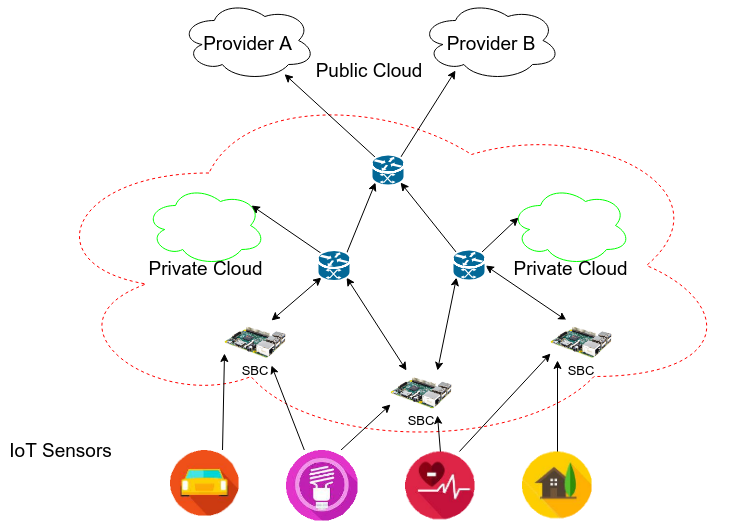
\includegraphics[width=0.4\textwidth]{figures/cassalesimgs-000.png}
%     &
%     asdfasdfa
%     % 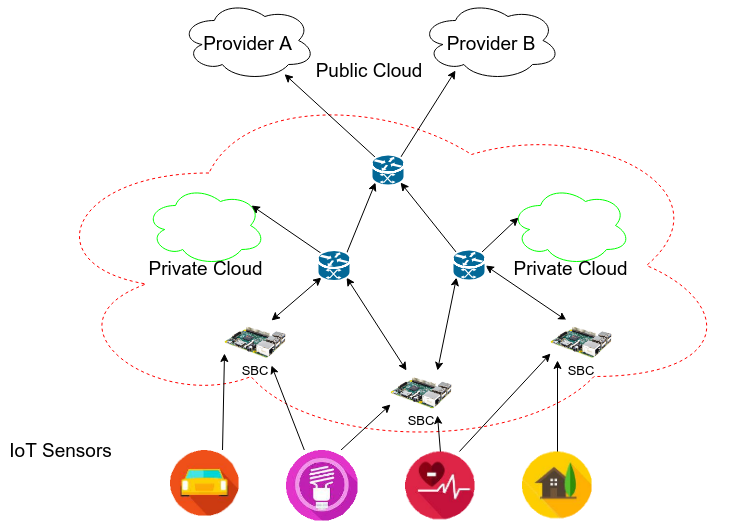
\includegraphics[width=0.4\textwidth]{figures/cassalesimgs-000.png}
% \end{tabular}


% {\begin{algorithm}[h]
% {\tiny 
% \begin{algorithm}
%     \DontPrintSemicolon
%     \SetKwFunction{FMain}{Main}
%     \SetKwProg{Fn}{algorithm}{:}{}
%     \Fn{\FMain{$f$, $a$, $b$, $\varepsilon$}}{
%           a\;
%           b\;
%           \KwRet\;
%     }
%     \;
%     \SetKwProg{Pn}{algorithm}{:}{\KwRet}
%     \Pn{\FMain{$f$, $a$, $b$, $\varepsilon$}}{
%           a\;
%           b\;
%     }
% \end{algorithm}
% \IncMargin{1em}
\begin{algorithm}[h]

% \begin{multicols}{2}
    \SetKwProg{Function}{Function}{:}{}
    % \DontPrintSemicolon
    % \KwIn{sample, ModelSet, params as p}
    % \KwOut{Classified Sample}
    % 
    \SetKwData{CW}{cleaningWindow}
    \SetKwData{NDT}{noveltyDetectionTrigger}
    \SetKwData{MEPC}{minExamplesPerCluster}
    \SetKwData{NF}{noveltyFactor}
    % 
    % \KwSty{Parameters}: cleaningWindow as \CW,
    % noveltyDetectionTrigger as \NDT,
    % minExamplesPerCluster as \MEPC,
    % noveltyFactor as \NF\\
    % 
    \SetKwFunction{nearestCluster}{nearestCluster}
    \SetKwFunction{clustering}{clustering}
    \SetKwFunction{sizeOf}{sizeOf}
    \SetKwFunction{NoveltyDetection}{NoveltyDetection}
    \SetKwFunction{handleModelSleep}{moveToSleep}
    \SetKwFunction{removeOldSamples}{removeOldSamples}
    % 
    % \KwData{ UnkownSet $\leftarrow$ $\emptyset$, ModelSleepSet $\leftarrow$ $\emptyset$, lastCleanupTime $\leftarrow$ now() }
    % 
    \Function{\NoveltyDetection{Model, Samples}}{
        newModelSet $\leftarrow$ $\emptyset$\;
        \ForEach{cl in \clustering(Samples)}{
            \If{$|cl.sampleSet| \geq$ \MEPC}{
                (distance, near) $\leftarrow$ \nearestCluster(cl, Model)\;
                \eIf{distance $<$ near.radius $\times$ \NF}{
                    cl.label $\leftarrow$ near.label\;
                    cl.type $\leftarrow$ extension\;
                }{
                    cl.label $\leftarrow$ noveltyIndex\;
                    noveltyIndex $\leftarrow$ noveltyIndex $+ 1$\;
                    cl.type $\leftarrow$ novelty\;
                }
                Samples $\leftarrow$ Samples $\ominus$ cl.sampleSet\;
                newModelSet $\leftarrow$ newModelSet $\oplus$ cl\;
            }
        }
        \Return{newModelSet}
    }
    \label{alg:MINAS-nd}
    \caption{Minas: Novelty Detection task.}
\end{algorithm}
\begin{algorithm}
    \SetKwProg{function}{Function}{:}{}
    % \DontPrintSemicolon
    % \KwIn{sample, ModelSet, params as p}
    % \KwOut{Classified Sample}
    % 
    \SetKwData{CW}{cleaningWindow}
    \SetKwData{NDT}{noveltyDetectionTrigger}
    \SetKwData{MEPC}{minExamplesPerCluster}
    \SetKwData{NF}{noveltyFactor}
    % 
    % \KwSty{Parameters}: cleaningWindow as \CW,
    % noveltyDetectionTrigger as \NDT,
    % minExamplesPerCluster as \MEPC,
    % noveltyFactor as \NF\\
    % 
    \SetKwFunction{nearestCluster}{nearestCluster}
    \SetKwFunction{clustering}{clustering}
    \SetKwFunction{sizeOf}{sizeOf}
    \SetKwFunction{NoveltyDetection}{NoveltyDetection}
    \SetKwFunction{handleModelSleep}{moveToSleep}
    \SetKwFunction{removeOldSamples}{removeOldSamples}
    % 
    \SetKwProg{algorithm}{algorithm}{:}{}
    \SetKwFor{With}{with}{}{}
    \SetKw{continue}{continue}
    % 
    \SetKwData{CW}{CW}
    \SetKwData{noveltyDetectionTrigger}{NDT}
    \SetKwData{MEPC}{MEPC}
    \SetKwData{NF}{NF}
    \SetKwData{mpiSize}{mpiSize}
    \SetKwData{mpiRank}{mpiRank}
    \SetKwData{EndOfStream}{EndOfStream}
    % 
    \KwIn{ModelSet, Sample Stream}
    \KwOut{Classified Stream as $out$}
    \SetKwFunction{MinasOnline}{MinasOnline}
    \function{\MinasOnline{ModelSet, SampleStream}}{
        UnkownSet $\leftarrow$ $\emptyset$, ModelSleepSet $\leftarrow$ $\emptyset$ \;
        lastCleanup $\leftarrow 0$ , noveltyIndex $\leftarrow 0$\;
        % sampleIn $\leftarrow 0$\;
        \ForEach{ {$sample_{i}$} $\in$ SampleStream }{
            % sample.label $\leftarrow$ unknown\;
            % (distance, cluster) $\leftarrow$ \nearestCluster(sample, ModelSet)\;
            nearest $\leftarrow$ \nearestCluster(sample, ModelSet)\;
            \eIf{nearest.distance $<$ nearest.cluster.radius}{
                sample.label $\leftarrow$ nearest.cluster.label\;
                nearest.cluster.lastUsed $ \leftarrow i $ \;
                % $out \leftarrow$ sample\;
                % outputStream.append(sample);
                % \textbf{continue};
                % \Return sample\;
            }
            {
                sample.label $\leftarrow$ unknown\;
                UnkownSet $\leftarrow$ UnkownSet $\cup$ sample\;
                \If{$|UnkownSet| \geq$ \NDT}{
                    % \tcc{Novelty Detection}
                    novelties $\leftarrow$ \NoveltyDetection(ModelSet $\cup$ ModelSleepSet, *UnkownSet)\;
                    ModelSet $\leftarrow$ ModelSet $\cup$ novelties\;
                }
                \If{ $ i > $ ( lastCleanup $ + $ \CW )}{
                    ModelSet $\leftarrow$ \handleModelSleep(ModelSet, *ModelSleepSet, lastCleanup)\;
                    UnkownSet $\leftarrow$ \removeOldSamples(UnkownSet, lastCleanup)\;
                    lastCleanup $ \leftarrow i $\;
                }
                % \Return sample\;
            }
            outputStream.append(sample);
            % $out \leftarrow$ sample\;
        }
    }
% \end{multicols}
% }
\label{alg:MINAS}
\caption{Our interpretation of MINAS \cite{faria2013novelty,Faria2016minas,Cassales2019a}}
\end{algorithm}
% \DecMargin{1em}


% --------------------------------------------------------------------------------------------------

% \begin{algorithm}[ht]
%   \caption{MINAS \cite{Faria2016minas,Cassales2019a}}
%   \label{alg:MINAS}
%   \renewcommand{\algorithmicrequire}{\textbf{Entrada:}}
%   \begin{algorithmic}[1]
%     %T $\leftarrow$ limiar de distância para pertencer ao grupo
%     %P $\leftarrow$ tempo de "inatividade" para passar para memória sleep
%     %ts $\leftarrow$ limiar para remoção de exemplos da memória temporária
%     \REQUIRE $Modelo,FCD,T,NumMinExemplos,ts,P$
%     \STATE $MemTmp \leftarrow \emptyset$
%     \STATE $MemSleep \leftarrow \emptyset$
%     \FORALL{$exemplo \in FCD$}
%     \STATE $(Dist,micro) \leftarrow$ micro-mais-proximo($exemplo,Modelo$)
%     \IF{$Dist < $ raio($micro$)}
%     \STATE $exemplo.classe \leftarrow micro.rotulo$
%     \STATE atualizar-micro($micro,exemplo$)
%     \ELSE
%     \STATE $exemplo.classe \leftarrow desconhecido$
%     \STATE $MemTmp \leftarrow MemTmp \cup exemplo$
%     \IF{$|MemTmp| \geq NumMinExemplos$}
%     \STATE $Modelo \leftarrow $ deteccao-novidade($Modelo,MemTmp,T$)
%     \ENDIF
%     \ENDIF
%     \STATE $TempoAtual \leftarrow exemplo.T$
%     \IF{$TempoAtual$ mod $TamJanela == 0$}
%     \STATE $Modelo \leftarrow$ mover-micro-grupos-mem-sleep($Modelo,MemSleep,P$)
%     \STATE $MemTmp \leftarrow$ remover-exemplos-antigos($MemTmp,ts$)
%     \ENDIF
%     \ENDFOR
%   \end{algorithmic}
% \end{algorithm}

% \begin{algorithm}[ht]
%   \caption{MINAS \cite{Faria2016minas,Cassales2019a}}
%   \label{alg:MINAS}
%   \renewcommand{\algorithmicrequire}{\textbf{Entrada:}}
%   \begin{algorithmic}[1]
%   \IF{root}
%     \WHILE{true}
%     \IF{can_read(S)}
%     input(S, $s$)
%     send(s, i++)
%     \ENDIF
%     \IF{can_rcv($(s, l)$, any)}
%         output($(s, l)$)
%         \IF{$l == '-'$ )}
%             store($(s, l)$, unknowns)
%             % \IF{$|MemTmp| \geq NumMinExemplos$}
%             % \STATE $Modelo \leftarrow $ deteccao-novidade($Modelo,MemTmp,T$)
%             % \ENDIF
%             % \ENDIF
%             % \STATE $TempoAtual \leftarrow exemplo.T$
%             % \IF{$TempoAtual$ mod $TamJanela == 0$}
%             % \STATE $Modelo \leftarrow$ mover-micro-grupos-mem-sleep($Modelo,MemSleep,P$)
%             % \STATE $MemTmp \leftarrow$ remover-exemplos-antigos($MemTmp,ts$)
%             % \ENDIF
%         \ENDIF
%     \ENDIF
%   \ENDWHILE
%   \ENDIF
%   \IF{leaf}
%     rcv($s$, root)
%     $l$ $\leftarrow$ classify($s$)
%     send($(s, l)$, root)
%   \ENDIF
%   \end{algorithmic}
% \end{algorithm}

% \begin{algorithm}
%   \caption{High level parallel algorithm}
%   \label{alg:highlevel-new}
%   \begin{algorithmic}[1]
%     \State {\bf Input}: an ensemble $E$, $num\_threads$, a data stream $S$
%     \State $P \gets Create\_service\_thread\_pool(num\_threads)$
%     \State $T \gets Create\_trainers\_collection(E)$
%     \For {each arriving instance $I$ in stream $S$}
%     \State $E$.classify($I$)
%     \For  {each trainer $T_i$ in trainers $T$} 
%     \State $k \gets poisson(\lambda)$
%     \State $T_i.update(I, k)$
%     \EndFor
%     \For {all trainers $T$} {\bf in parallel}
%     \State $W\_inst \gets I * k$
%     \State $Train\_on\_instance(W\_inst)$
%     \EndFor
%     \If {change detected}
%     \State $reset\_classifier$
%     \EndIf
%     \EndFor
%   \end{algorithmic}
% \end{algorithm}

 }
% \label{alg:MINAS}
% \caption{Our interpretation of MINAS \cite{faria2013novelty,Faria2016minas,Cassales2019a}}
% \end{algorithm}}

% \begin{figure}[ht]
%     \subfloat[Percentage storage utilization]{
%         \begin{minipage}[c][1\width]{0.4\textwidth}
%         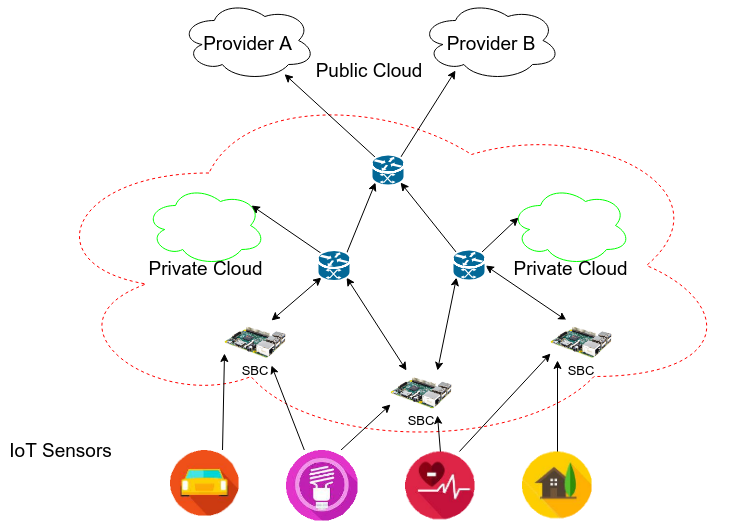
\includegraphics[width=1.1\textwidth]{figures/cassalesimgs-000.png}
%         \end{minipage}}
%     %   \begin{minipage}[c][1\width]{0.5\textwidth}
%     %     %  \includegraphics[width=1\textwidth]{image_file_name}
%     %     \begin{algorithm}[h]
%     %     % {\tiny 
% \begin{algorithm}
%     \DontPrintSemicolon
%     \SetKwFunction{FMain}{Main}
%     \SetKwProg{Fn}{algorithm}{:}{}
%     \Fn{\FMain{$f$, $a$, $b$, $\varepsilon$}}{
%           a\;
%           b\;
%           \KwRet\;
%     }
%     \;
%     \SetKwProg{Pn}{algorithm}{:}{\KwRet}
%     \Pn{\FMain{$f$, $a$, $b$, $\varepsilon$}}{
%           a\;
%           b\;
%     }
% \end{algorithm}
% \IncMargin{1em}
\begin{algorithm}[h]

% \begin{multicols}{2}
    \SetKwProg{Function}{Function}{:}{}
    % \DontPrintSemicolon
    % \KwIn{sample, ModelSet, params as p}
    % \KwOut{Classified Sample}
    % 
    \SetKwData{CW}{cleaningWindow}
    \SetKwData{NDT}{noveltyDetectionTrigger}
    \SetKwData{MEPC}{minExamplesPerCluster}
    \SetKwData{NF}{noveltyFactor}
    % 
    % \KwSty{Parameters}: cleaningWindow as \CW,
    % noveltyDetectionTrigger as \NDT,
    % minExamplesPerCluster as \MEPC,
    % noveltyFactor as \NF\\
    % 
    \SetKwFunction{nearestCluster}{nearestCluster}
    \SetKwFunction{clustering}{clustering}
    \SetKwFunction{sizeOf}{sizeOf}
    \SetKwFunction{NoveltyDetection}{NoveltyDetection}
    \SetKwFunction{handleModelSleep}{moveToSleep}
    \SetKwFunction{removeOldSamples}{removeOldSamples}
    % 
    % \KwData{ UnkownSet $\leftarrow$ $\emptyset$, ModelSleepSet $\leftarrow$ $\emptyset$, lastCleanupTime $\leftarrow$ now() }
    % 
    \Function{\NoveltyDetection{Model, Samples}}{
        newModelSet $\leftarrow$ $\emptyset$\;
        \ForEach{cl in \clustering(Samples)}{
            \If{$|cl.sampleSet| \geq$ \MEPC}{
                (distance, near) $\leftarrow$ \nearestCluster(cl, Model)\;
                \eIf{distance $<$ near.radius $\times$ \NF}{
                    cl.label $\leftarrow$ near.label\;
                    cl.type $\leftarrow$ extension\;
                }{
                    cl.label $\leftarrow$ noveltyIndex\;
                    noveltyIndex $\leftarrow$ noveltyIndex $+ 1$\;
                    cl.type $\leftarrow$ novelty\;
                }
                Samples $\leftarrow$ Samples $\ominus$ cl.sampleSet\;
                newModelSet $\leftarrow$ newModelSet $\oplus$ cl\;
            }
        }
        \Return{newModelSet}
    }
    \label{alg:MINAS-nd}
    \caption{Minas: Novelty Detection task.}
\end{algorithm}
\begin{algorithm}
    \SetKwProg{function}{Function}{:}{}
    % \DontPrintSemicolon
    % \KwIn{sample, ModelSet, params as p}
    % \KwOut{Classified Sample}
    % 
    \SetKwData{CW}{cleaningWindow}
    \SetKwData{NDT}{noveltyDetectionTrigger}
    \SetKwData{MEPC}{minExamplesPerCluster}
    \SetKwData{NF}{noveltyFactor}
    % 
    % \KwSty{Parameters}: cleaningWindow as \CW,
    % noveltyDetectionTrigger as \NDT,
    % minExamplesPerCluster as \MEPC,
    % noveltyFactor as \NF\\
    % 
    \SetKwFunction{nearestCluster}{nearestCluster}
    \SetKwFunction{clustering}{clustering}
    \SetKwFunction{sizeOf}{sizeOf}
    \SetKwFunction{NoveltyDetection}{NoveltyDetection}
    \SetKwFunction{handleModelSleep}{moveToSleep}
    \SetKwFunction{removeOldSamples}{removeOldSamples}
    % 
    \SetKwProg{algorithm}{algorithm}{:}{}
    \SetKwFor{With}{with}{}{}
    \SetKw{continue}{continue}
    % 
    \SetKwData{CW}{CW}
    \SetKwData{noveltyDetectionTrigger}{NDT}
    \SetKwData{MEPC}{MEPC}
    \SetKwData{NF}{NF}
    \SetKwData{mpiSize}{mpiSize}
    \SetKwData{mpiRank}{mpiRank}
    \SetKwData{EndOfStream}{EndOfStream}
    % 
    \KwIn{ModelSet, Sample Stream}
    \KwOut{Classified Stream as $out$}
    \SetKwFunction{MinasOnline}{MinasOnline}
    \function{\MinasOnline{ModelSet, SampleStream}}{
        UnkownSet $\leftarrow$ $\emptyset$, ModelSleepSet $\leftarrow$ $\emptyset$ \;
        lastCleanup $\leftarrow 0$ , noveltyIndex $\leftarrow 0$\;
        % sampleIn $\leftarrow 0$\;
        \ForEach{ {$sample_{i}$} $\in$ SampleStream }{
            % sample.label $\leftarrow$ unknown\;
            % (distance, cluster) $\leftarrow$ \nearestCluster(sample, ModelSet)\;
            nearest $\leftarrow$ \nearestCluster(sample, ModelSet)\;
            \eIf{nearest.distance $<$ nearest.cluster.radius}{
                sample.label $\leftarrow$ nearest.cluster.label\;
                nearest.cluster.lastUsed $ \leftarrow i $ \;
                % $out \leftarrow$ sample\;
                % outputStream.append(sample);
                % \textbf{continue};
                % \Return sample\;
            }
            {
                sample.label $\leftarrow$ unknown\;
                UnkownSet $\leftarrow$ UnkownSet $\cup$ sample\;
                \If{$|UnkownSet| \geq$ \NDT}{
                    % \tcc{Novelty Detection}
                    novelties $\leftarrow$ \NoveltyDetection(ModelSet $\cup$ ModelSleepSet, *UnkownSet)\;
                    ModelSet $\leftarrow$ ModelSet $\cup$ novelties\;
                }
                \If{ $ i > $ ( lastCleanup $ + $ \CW )}{
                    ModelSet $\leftarrow$ \handleModelSleep(ModelSet, *ModelSleepSet, lastCleanup)\;
                    UnkownSet $\leftarrow$ \removeOldSamples(UnkownSet, lastCleanup)\;
                    lastCleanup $ \leftarrow i $\;
                }
                % \Return sample\;
            }
            outputStream.append(sample);
            % $out \leftarrow$ sample\;
        }
    }
% \end{multicols}
% }
\label{alg:MINAS}
\caption{Our interpretation of MINAS \cite{faria2013novelty,Faria2016minas,Cassales2019a}}
\end{algorithm}
% \DecMargin{1em}


% --------------------------------------------------------------------------------------------------

% \begin{algorithm}[ht]
%   \caption{MINAS \cite{Faria2016minas,Cassales2019a}}
%   \label{alg:MINAS}
%   \renewcommand{\algorithmicrequire}{\textbf{Entrada:}}
%   \begin{algorithmic}[1]
%     %T $\leftarrow$ limiar de distância para pertencer ao grupo
%     %P $\leftarrow$ tempo de "inatividade" para passar para memória sleep
%     %ts $\leftarrow$ limiar para remoção de exemplos da memória temporária
%     \REQUIRE $Modelo,FCD,T,NumMinExemplos,ts,P$
%     \STATE $MemTmp \leftarrow \emptyset$
%     \STATE $MemSleep \leftarrow \emptyset$
%     \FORALL{$exemplo \in FCD$}
%     \STATE $(Dist,micro) \leftarrow$ micro-mais-proximo($exemplo,Modelo$)
%     \IF{$Dist < $ raio($micro$)}
%     \STATE $exemplo.classe \leftarrow micro.rotulo$
%     \STATE atualizar-micro($micro,exemplo$)
%     \ELSE
%     \STATE $exemplo.classe \leftarrow desconhecido$
%     \STATE $MemTmp \leftarrow MemTmp \cup exemplo$
%     \IF{$|MemTmp| \geq NumMinExemplos$}
%     \STATE $Modelo \leftarrow $ deteccao-novidade($Modelo,MemTmp,T$)
%     \ENDIF
%     \ENDIF
%     \STATE $TempoAtual \leftarrow exemplo.T$
%     \IF{$TempoAtual$ mod $TamJanela == 0$}
%     \STATE $Modelo \leftarrow$ mover-micro-grupos-mem-sleep($Modelo,MemSleep,P$)
%     \STATE $MemTmp \leftarrow$ remover-exemplos-antigos($MemTmp,ts$)
%     \ENDIF
%     \ENDFOR
%   \end{algorithmic}
% \end{algorithm}

% \begin{algorithm}[ht]
%   \caption{MINAS \cite{Faria2016minas,Cassales2019a}}
%   \label{alg:MINAS}
%   \renewcommand{\algorithmicrequire}{\textbf{Entrada:}}
%   \begin{algorithmic}[1]
%   \IF{root}
%     \WHILE{true}
%     \IF{can_read(S)}
%     input(S, $s$)
%     send(s, i++)
%     \ENDIF
%     \IF{can_rcv($(s, l)$, any)}
%         output($(s, l)$)
%         \IF{$l == '-'$ )}
%             store($(s, l)$, unknowns)
%             % \IF{$|MemTmp| \geq NumMinExemplos$}
%             % \STATE $Modelo \leftarrow $ deteccao-novidade($Modelo,MemTmp,T$)
%             % \ENDIF
%             % \ENDIF
%             % \STATE $TempoAtual \leftarrow exemplo.T$
%             % \IF{$TempoAtual$ mod $TamJanela == 0$}
%             % \STATE $Modelo \leftarrow$ mover-micro-grupos-mem-sleep($Modelo,MemSleep,P$)
%             % \STATE $MemTmp \leftarrow$ remover-exemplos-antigos($MemTmp,ts$)
%             % \ENDIF
%         \ENDIF
%     \ENDIF
%   \ENDWHILE
%   \ENDIF
%   \IF{leaf}
%     rcv($s$, root)
%     $l$ $\leftarrow$ classify($s$)
%     send($(s, l)$, root)
%   \ENDIF
%   \end{algorithmic}
% \end{algorithm}

% \begin{algorithm}
%   \caption{High level parallel algorithm}
%   \label{alg:highlevel-new}
%   \begin{algorithmic}[1]
%     \State {\bf Input}: an ensemble $E$, $num\_threads$, a data stream $S$
%     \State $P \gets Create\_service\_thread\_pool(num\_threads)$
%     \State $T \gets Create\_trainers\_collection(E)$
%     \For {each arriving instance $I$ in stream $S$}
%     \State $E$.classify($I$)
%     \For  {each trainer $T_i$ in trainers $T$} 
%     \State $k \gets poisson(\lambda)$
%     \State $T_i.update(I, k)$
%     \EndFor
%     \For {all trainers $T$} {\bf in parallel}
%     \State $W\_inst \gets I * k$
%     \State $Train\_on\_instance(W\_inst)$
%     \EndFor
%     \If {change detected}
%     \State $reset\_classifier$
%     \EndIf
%     \EndFor
%   \end{algorithmic}
% \end{algorithm}

 }
%     %     \SetAlgoVlined
%     %     \KwIn{sample, ModelSet, params as p}
%     %     \label{alg:MINAS}
%     %     \caption{Our interpretation of MINAS \cite{faria2013novelty,Faria2016minas,Cassales2019a}}
%     %     \end{algorithm}
%     %   \end{minipage}}
%    \hfill
%     \subfloat[standard deviation]{
%       \begin{minipage}[c][1\width]{0.4\textwidth}
%     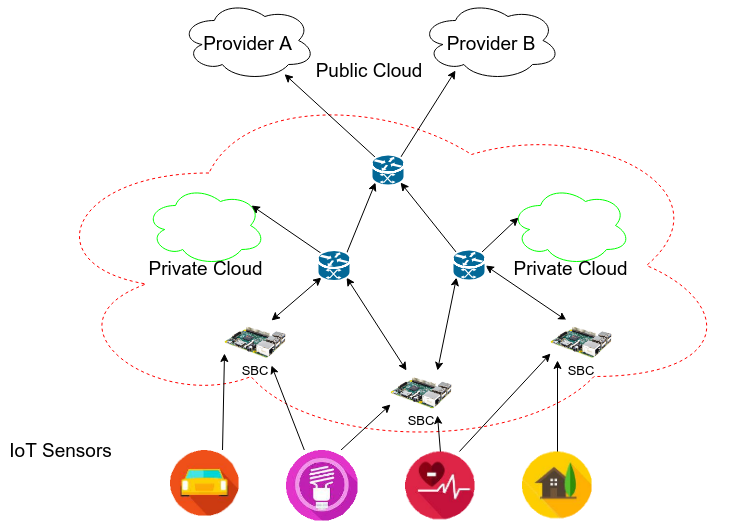
\includegraphics[width=1.1\textwidth]{figures/cassalesimgs-000.png}
%       \end{minipage}}
%   \caption{}
% \end{figure}%\FloatBarrier

\section{Proposal}
\label{sec:prop}
% Proposal:
%  - retomar problema {iot, sec, ND};
%  - objetivo;
%  - soluções {MINAS, paralelismo, distribuído, ~~py-kafka, flink,~~ mpi}
%  - propor uma solução

% \begin{highlight}
% A expansão do IoT na industria e vida diária\\
% leva a maior incidência de intrusão e subversão\\
% portanto são necessários sistemas de detectão de intrusão\\
% eficases (boa acuracia) e eficientes (baixa latência)\\
% portanto propôen-se\\
% um NIDS que utiliza algoritmo de detecção de novidades (para acurárcia)\\
% implementado de maneira distruída na borda e nuvem (para latência).\\
% \end{highlight}

%Amid of \iot expansion in multiple fields, from industry to daily life, the constant threat of intrusion
% , subversion (overthrow), denial of service (or any other unexpected detrimental behavior)
% by any component of a system or external actors is a prospect looming over many systems administrators and for that reason
% Thus,  new network surveillance tools are needed, especially effective (accurate) and efficient (fast reaction and good throughput) \nids.
% Following that reasoning, new \nids and other autonomous and analytic system
% surveillance tools are being proposed, many employing techniques such as Anomaly
% and Novelty Detection.
% These tools require the network packet traffic to be constantly analysed,

% Este apresenta uma proposta de implementação distribuida do MINAS que segue as diretrizes da arquitetura IDSA-IoT, atendendo aos seguintes requisitos:
% (i) a etapa de classificação de vários fluxos deve ocorrer em paralelo, sendo processada em diversos locais físicos da arquitetura 
% (ii) a etapa de detecção de novidades (evolução do modelo) deve ocorrer em paralelo, sendo processada em diversos locais físicos da arquitetura 
% (iii)  as duas etapas anteriores, por sua vez também deverão ser executadas paralelamente, podendo ocorrer em partes distintas do sistema
% (iv) possa ser implementada em dispositivos com recursos limitados 

% acho que falta casar melhor esse começo com a estória contada no abstract... - helio
% 
% In this work we investigate an appropriate architecture for performing \nd at
% the edge, as a means of allowing small IoT devices to filter undesirable network
% traffic.
% Our approach is based on the \arch architecture \cite{Cassales2019a} and \nd
% techniques provide by the \minas algorithm \cite{Faria2016minas}. Named \mfog,
% our distributed algorithm explores load balancing to enable low profile devices
% at the edge of the net to also work on the classification and detection of
% unwanted traffic.
% 
% eu trocaria a frase abaixo pelas 2 acima - helio

In this work we investigate an appropriate architecture for performing \nd at
the edge, allowing small IoT devices to detect undesirable network behavior.
To that end, we propose and evaluate \mfog, a distributed \nd system following
the \arch architecture \cite{Cassales2019a} and based on a distributed version
of the algorithm \minas \cite{Faria2016minas}.
Our approach explores distributed computing and a trivial load balancer to
enable low profile devices to classify and detect unwanted traffic in a
scalable, edge focused way.

% Hermes:
% In this work we propose and assess MFOG, a distributed data stream
% novelty detection system based on the algorithm MINAS for securing IoT networks.
% MFOG implements a distributed version of MINAS according to the IDSA-IoT
% architecture proposed in a previous work [ ], to execute in the edge where small
% devices and constrained resources may be prevalent

% In this work we investigate the application of the \arch architecture
% \cite{Cassales2019a} with \nd techniques by use of \minas algorithm
% \cite{Faria2016minas}, by implementation and evaluation of a parallel and
% distributed descendant of those two works we named \mfog.
However, given the distributed nature and the typical use of small computing
devices in IoT scenarios as well as the need handle network speeds, new challenges arise:
\begin{enumerate*}[label=(\emph{\roman*})]
  \item the classification phase of the algorithm must occur in parallel at
  different nodes;
  \item the novelty detection phase, which provides the model evolution, must
  also be asynchronous;
  \item the algorithm complexity (time and space) must allow it to be processed
  by modest computing devices (i.e., small memory and low processor performance).
\end{enumerate*}

% \todo{Relembrar ids-iot, fase offline e online}
% Thus we propose a \nids using MINAS \cite{Faria2016minas}
% % (a Novelty Detection algorithm)
% to effectively identify previous and new intrusion threats,
% implemented by following the  architecture \cite{Cassales2019a} using parallel and distributed techniques leveraging
% edge and cloud for efficient computing.

% {\color{red} introdução?}
% \todo{[start] intro/related?}
% Hermes:
% O foco é detecção de intrusão ou detecção de novidade? Não sei se ND consegue de
% fato detectar intrusão e acho que esse é um terreno pantanoso.
% Se quiser citar a vasta literatura sobre IDS tudo bem, mas falar de IDS dentro
% da proposta pode dar uma ideia errada sobre a proposta.
% Sugestão:
% Our objective is to detect novel and emerging patterns in the network traffic
% and possible misbehavior (e.g., novel and emerging misbehavior that cannot be
% detected by misuse-based IDS systems) ....
\nids 
monitor network traffic, and analyze the characteristics of each flow 
% aggregated into flow descriptors and further processed in a classification
% analyze 
to identify any intrusion or misbehavior.
% using methods such as classification and Novelty Detection
% This requirement in turn, requesting more computing power at the edge.
% While requesting more computing power in a cloud environment is trivial and
% inexpensive, the same cannot be said 
However, this problem requires both fast and accurate response \cite{DaCosta2019a}:
fast response is needed to have a proper reaction before harm can be cast
to the network and to cope with the traffic without imposing loss or delay
in the \nids or observed network;
accurate response is required as not to misidentify,
% harmless with harmful and vice-versa,
especially the case of false positive that leads to false alarms.
To achieve those goals, we leverage fog computing.

% \hl{intro/related?}

In common \iot scenarios, data is captured by small devices and sent to the
cloud for any compute or storage tasks, but this is not feasible in a \nids
scenario.
% Even though we also capture data produced in the edge, sending this data to the
% cloud would in the worst case double the internet communication requirements of
% the overall system.
Fog computing infrastructure aims to offload processing from the cloud
providers by placing edge devices closer to end-users and/or data sources.
% But two \minas steps limit this fog offload, the processing intensive novelty
% detection and, long term model storage and distribution of the internal model.
% Those steps surpass the capabilities of common fog hardware and therefore need
% to be at least shared to a cloud where such requirements are easy and cheap to
% fulfill.

% \todo{[end] intro/related?}

In our proposal, fog and cloud computing resources are combined to minimize
the time elapsed between a flow descriptor ingestion and intrusion alarm,
% Melhor falar da proposta em nivel mais abstarto, destacando O QUE se
% quer, deixando o COMO é implementado para mais tarde. Ou
% seja, que aqui ainda é cedo para falar de MPI.
performing the classification step of \minas  running multiple
classifier instances.
After the initial classification, the resulting label can be used immediately,
but if the sample is labeled as \emph{unknown}, this sample must be stored and
the novelty detection step will be triggered.
% , and those steps require more
% resources and thus are divided in fog and cloud.

% Therefore, our objective is a Distributed novelty detection in streams using limited hardware.
% Previous attempts to attain the objective of distributed fast


% visão geral de iot nessa fig
% quais redes envolvidas
% processamento extra na borda
To have a better overview of our proposal and how it integrates with existing
\iot environments, Figure \ref{fig:mfog-phy-arch-cloud} depicts such scenario
showing from bottom to top:
\iot devices directly connected to a (local) gateway network;
this gateway network could be as simple as a single Internet router 
or be more complex by connecting to private clouds or 
containing more devices providing fog computing capabilities;
lastly, available over the internet, the traditional public cloud provides
inexpensive computing and storage on demand.
% \todo{the following is needed?}
% {
% In this scenario, the further apart resources are, more network
% resources need to be employed, and, as with any networked system, the
% latency increases.
In this scenario, the further apart resources are, the more network
resources need to be employed, and, as with any networked system, the
higher is the latency.
% E como pretende lidar/evitar alta latencia?
% }

\begin{figure}[hb]
  \centering
  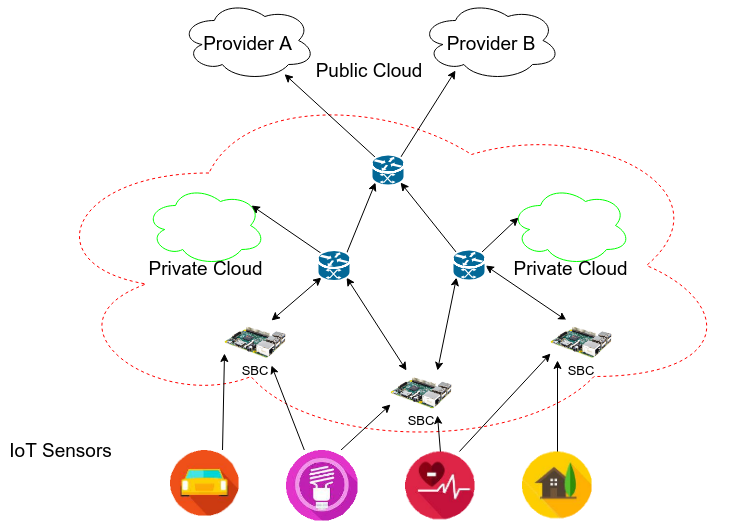
\includegraphics[width=0.5\linewidth]{figures/cassalesimgs-000.png}
  \caption{\arch \cite{Cassales2019a} physical architecture and deployment
  scenario overview.}
  \label{fig:mfog-phy-arch-cloud}
\end{figure}

% \begin{figure*}[hbt]
%   \centerline{
%     \begin{subfigure}{.5\textwidth}
%       \centering
%       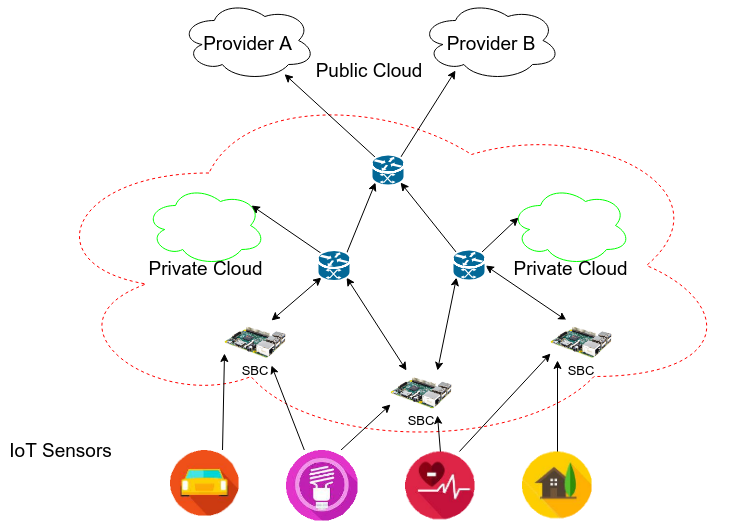
\includegraphics[width=1.0\linewidth]{figures/cassalesimgs-000.png}
%       \caption{\arch physical architecture and deployment scenario overview
%       from \cite{Cassales2019a}.}
%       \label{fig:mfog-phy-arch-cloud}
%     \end{subfigure}
%     \begin{subfigure}{.5\textwidth}
%       \centerline{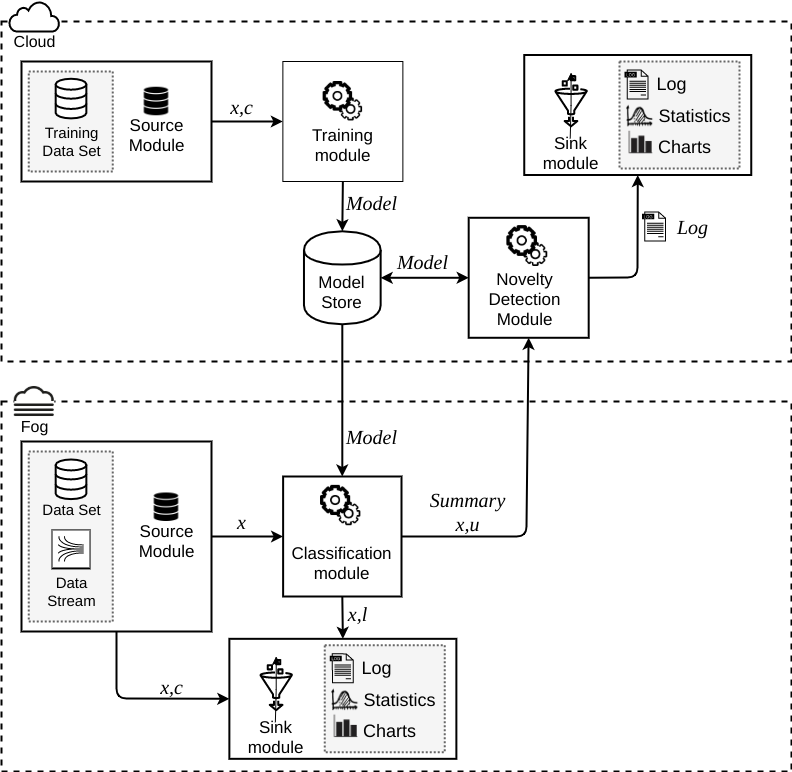
\includegraphics[width=0.95\linewidth]{figures/mfog-arch-v2_en.png}}
%       \caption{\mfog components and communications overview, }
%       \label{fig:mfog-architecture}
%     \end{subfigure}
%   }
%   \caption{Architecture overview.}
%   \label{fig:arch-overview}
% \end{figure*}

%   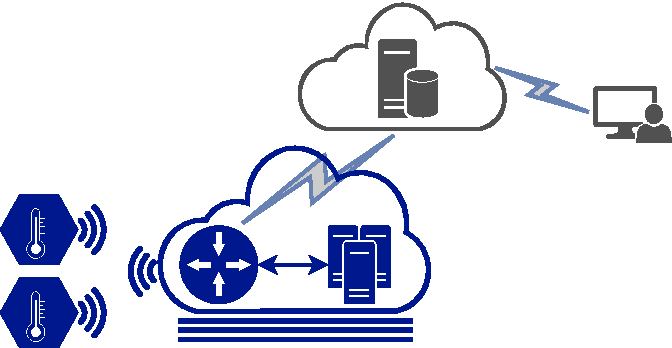
\includegraphics[width=0.9\linewidth,page=1]{figures/mfog-arch-fisica.svg.pdf}
% The overall organization of components, connections and interactions with external
% actors is shown in Figure \ref{fig:mfog-phy-arch-cloud},
% from bottom left to top right: sensor network; fog containing gateway router
% and novelty detection cluster; cloud storage for model, alarms and statistics
% and; human supervisor addressing alarms and statistics.

% While our proposal focuses on fog computing resources, those resources are often limited
% and they do not have the same reach and availability as traditional public cloud.
% For that reason we also leverage the public cloud for model storage and distribution,
% global novelty detection and alarm forwarding.

% % In Figure \ref{fig:mfog-architecture} we depict 
% The overall \mfog architecture can be cut down to individual modules:
% three main functional modules, being the Classification and Novelty
% % three main functional modules being Training, Classification and Novelty
% Detection handling \minas main tasks.
% % Three auxiliary Source, Sink and Model Store, addressing external and
% % internal connections as well as providing facilities to our tests and
% % experiments.

% The overall \mfog architecture has two main modules, Classification and Novelty
% Detection, handling \minas main tasks.

% enumerar módulos e funções
% \\descrever etapas do \minas e onde se encaixa
% \\descrever onde módulos são multiplexados
% \\descrever casos de muiltiplos fluxos (redes locais)

% \todo{Needs review}
% Source Module provides the input data stream for Offline and Online phases of \minas
% and is deployed in cloud and in fog for each respective phase and a variant for
% testing on our experiments.
% Model Store is another trivial module handling the initial Model storage and distribution
% for Classification and Novelty Detection modules.
% Last of the auxiliary modules is the Sink module, it denotes the consumer of labeling
% output stream such as an alarm system, however in our implementation it is much more
% complex, handling all tests metrics extraction and evaluations for our experiments,
% aggregating all output (stream and logs) in files for proper analysis and later comparisons.
% This module also differs in its software stack from the C language and MPI library,
% for the ease of implementing such analysis needed by our experiments, 
% courtesy of Pandas and NumPy libraries, we employed Python for this module.


% Training Module encapsulates the Offline phase of \minas and its output, being the
% initial model, is stored by the Model Store.

The overall \mfog architecture has two main modules, Classification and Novelty
Detection, which implement the \minas main tasks.
The Classification Module performs the same task of the \minas Online phase and
is the focal point for parallelism and distribution in our proposal.
It is replicated in the fog and runs on each cluster node, using a configurable
number of threads (limited to the node CPU core count).
% with one or more nodes and each node multiple processes (limited to the individual CPU core count).

The Novelty Detection Module can also be replicated,
the choice being one instance per local network, one global cloud instance,
or both.
This module also handles the homonymous task of \minas Online phase, receiving
all the samples labeled with \emph{unknown}, storing them in an internal
\emph{unknown-buffer}, and, when this buffer is full, performing the \minas
Novelty Detection task (clustering followed by validation).

% In Figure \ref{fig:mfog-architecture} we depict each logical component associated
% with each \minas step and its communications, we also depict extra modules for sampling
% and measurements.
% Each communication in Figure \ref{fig:mfog-architecture} shows the direction of the data flow
% and identifies the data contained:
% $Model$ is \minas internal Model containing a set of cluster data structures,
% $x,c$ identifies a sample with the real class,
% $x$ is the sample without the real class,
% $x,l$ identifies a sample with the assigned label,
% $x,u$ is  sample with the \emph{unknown} label,
% $summary$ is a statistical summary of model usage.

\subsection{Policies}\label{sec:policies}

% achei confuso o uso de "opens data distribution..."
The design of our distributed \nd architecture includes partitioning the
functionalities of \minas and establishing the appropriate data flows
between different actors.
Changes to placement and behavior can have different impacts and should be
chosen with care.
% The distribution of steps and tasks in various modules opens data distribution
% and its impacts to discussion.
% 
% acho que falta deixar claro o que quer comparar...
% 
The decisions following these discussions can be organized in several policies,
some of them were recurring during our implementation discussions and are:

\begin{itemize}
  \item Regarding the allocation of the Novelty Detection Module:
  \begin{itemize}
    
    \item At each fog node: patterns will be only detected if sufficient samples
    of them occur in the local observed network, use of the local node
    processing power, and a model synchronization mechanism between networks
    must be added;

    \item In the cloud: detect patterns even when scattered on each local
    network, each sample with \emph{unknown} label must be sent from edge to
    cloud implying increased internet link usage and increased delay between the
    appearance of a pattern, its detection and propagation to fog classifiers;

    \item On both: local \emph{unknown} buffer is maintained and novelty
    detection is local as well, once a sample is considered as noise or outlier
    it shall be sent to the cloud where the process repeats but with global
    data.
    This choice needs an even more complex model synchronization mechanism.

  \end{itemize}
    
  \item Regarding the model cleanup (forget mechanism): Even when a global
  novelty detection is used, local models can be optimized for faster
  classification using the local model statistics by sorting by (or removing)
  least used clusters;

  \item Lastly, reclassification of \emph{unknowns}: In the novelty detection
  task in \minas, the \emph{unknown-buffer} is effectively classified
  using the new set of clusters.
  In Algorithm \ref{alg:MINAS-nd} line \ref{alg:MINAS-nd:reclassify}, the
  new valid cluster (novelty or extension) includes the set of samples composing
  that cluster, thus, if this new label assignment was put forth to the system
  output it would introduce delayed outputs, more recent and perhaps more
  accurate.
  Also, it would change the system data stream behavior from a \emph{map}
  (meaning each input has one output) to a \emph{flatMap} (each input can have
  many outputs).

\end{itemize}

% \begin{highlight}
% - Detecção de novidades e manutenção de modelo em ambiente distribuído:

%   - Mecanismo de ND local (síncrono) vs nuvem quanto à atraso de definição de modelo
%     (nesse ponto é onde a hipótese prevê maior diferença, grande ponto de interesse);

%   - Mecanismo de esquecimento local vs global (modelo único ou por nó);

%   - Atraso na reclassificação dos desconhecidos;
% \end{highlight}

\subsection{Implementation}\label{sec:implementation}

The original MINAS algorithm has a companion implementation\footnote{Available
at \url{http://www.facom.ufu.br/~elaine/MINAS}.} (\refminas) written in Java
using MOA library base algorithms such as K-means and CluStream, but our
implementation only used K-means.
% \refminas employs Java's double, a $64 bits$ number whose precision is not
% absolutely necessary and, as it is often necessary to shuffle between nodes via
% network and a small economy could be made with only a float number with $32 bits$.
Another difference between \refminas and \mfog is the definition of cluster radius
derived from the distances of elements forming the cluster and the cluster's center.
\refminas uses the maximum distance while \mfog uses the standard deviation
of all distances as described in \cite{Faria2016minas}.

% Desafios de implementação:
% <!--
% - Definição de raio: desvio padrão das distâncias versus distancia máxima;
% - Atualização do micro-cluster limita-se à atualização do atributo \texttt{T};
% - Remoção de exemplos na implementação de referência é feita somente para o algoritmo \textit{CluStream};
% - Inclusão de borda: algoritmo inclui ($<=$), referência não inclui ($<$);
% - Seguiu-se as mesmas divergências anteriores para comparação dos resultados com a implementação referência;
% - Inclusão da borda;
% - Comportamento do mecânismo de \textit{sleep-model} não está definido, portanto não está ativo;
% - Processo de clusterização é limitado ao algoritmo \textit{K-Means}. Algoritmo \textit{CluStream} não está implementado;
% - -->
% - `Double vs Float`:
%   - Na implementação de referência, java double é utilizado;
%   - Na nova implementação duas versões foram testadas e a diferença de precisão entre as duas é de `5 E-8`;
%   - **Solução:** Use `float32` e economize os bits já que haverá comunicação entre nós e módulos;
% - Formato do fluxo de saída:
%   - Implementação de referência utiliza a tripla `(id, classe, etiqueta)`;
%   - Primeira implementação em C utiliza `(id, clusterLabel, clusterId, clusterRadius, label, distance, secondDistance)`;
%   - Segunda implementação utiliza dupla `(id, label)`;
%   - Na etapa de avaliação, independente de versão, o fluxo original é lido;
%   - **Solução:** O formato mínimo é `(id, label)`;

\newcommand{\val}{$\vec{v}\,$\xspace}
The stream formats for input and output are also of note.
% <<<<<<< HEAD
% Input information needed is the sample value (\val),
% it being sequence of real numbers with length $d$ (dimension).
% In addition to \val, for evaluation and training purposes the class
% identifier as single character, and unique item identifier
% (\emph{uid}) can be provided or be the sample index in the stream.
% For output information and format the decision isn't so clear as we can't
% predict future system integrations needs.
% Some systems may require only novelty alarms (the minimal useful output),
% % or samples with label in a subset of all labels,
% other systems may require every sample with label and original \val.
% For the assessment in this work, \mfog outputs only enough information for
% evaluation with the full data set, meaning the format can be defined as a tuple
% containing \emph{uid} and assigned label.
% =======
As input, the algorithm takes samples (\val), which are a sequence of numbers
with dimension $d$.
In addition to \val, for both training and evaluation, the class
identifier is provided as a single character, along with a unique item identifier
(\emph{uid}), which can otherwise be determined from the sample index in the input stream.

% muito longo, difícil de entender... - helio
% For output information and format the decision isn't so clear as we can't
% predict future system integrations needs like only novelty alarms or every
% samples original \val with assigned label so, we have a compromise and put only
% enough information for the Sink Module (where the full information from the
% testing file or stream can be accessed) meaning the format can be defined as a
% tuple containing \emph{uid} and assigned label.
As its output, the algorithm returns the original sample \val followed by the
assigned label. Adjustments can easily be made to provide the output results as
a tuple containing \emph{uid} and the assigned label.

% >>>>>>> dd70e6dd2f93dbb63f7f84ee937aafc4b6ff9684

% - Reprocessamento dos exemplos utilizados para atualização do modelo:
%   - Muda o comportamento do operador de fluxo de `Map` para `Flatmap`, ou seja,
%     requer outro fluxo de saída para a transmissão de padrões novidade (alarmes);
%   - Para reclassificação a definição de raio é modificada de `r = f * σ` (fator
%     multiplicando desvio padrão) para `r = max(distance)` (distância máxima);
%   - Passível da crítica de *overfitting*. Isto é, este processo pode
%     inflar a métrica de precisão;
%   - **Solução:** *em aberto*;

% Another implementation decision related to the output stream is whether or not
% to reprocess, and add to the output stream, examples in the unknown buffer after
% the novelty detection procedure, meaning one item can be classified once as
% unknown and again with a label.
% Our preliminary tests using this technique had increased true positives when compared to
% not using it.
% However this changes the stream operator behavior from a \textit{Map} to a
% \textit{FlatMap} having duplicate entries on the output stream as previously
% mentioned.
% Regardless of choice the classification of the unknown buffer after a model
% update, using the full model or just the added set of clusters, is done to
% remove the examples ``consumed'' in the creation of a new cluster in the internals
% of the clustering algorithm.
% This removal can be made less complex if using only new clusters 

% Próximos desafios:
% - Distribuição e paralelização para minimização de latência entre novo item no fluxo e sua classificação:
%   - Tempo de passagem da instância pelo classificador;
%   - Volume máximo do sistema;
%   - Diferenças de precisão de acordo com a carga;

% <<<<<<< HEAD
% For \mfog, the Message Passing Interface (MPI, from \emph{Open MPI 4.0.4})
% library was used.
% In MPI programming, multiple processes of the same program are created by the
% run-time and each process instance receives a rank parameter.
% For \mfog this parameter indicate if the process is root, rank $0$, or leaf otherwise.
% Beyond this division, each process also operates two threads, for the root
% there is a sampler and detector threads, for the leafs each has a model receiver
% thread and multiple classifier threads.
% =======
% For \mfog, the Message Passing Interface (MPI, from \emph{Open MPI 4.0.4}) library was used.
% In MPI programming, multiple processes of the same program are created by the
% run-time and each process instance receives a rank parameter, for \mfog this
% parameters indicate if the process is root, rank $0$, or leaf otherwise.
% Beyond this division, each process also operates two threads, for the root
% there is a sampler and detector threads, for the leafs each has a model receiver
% thread and multiple classifier threads.

For evaluation purposes, an \mfog implementation\footnote{Available at
\url{https://github.com/luis-puhl/minas-flink}.} was made using MPI (\emph{Open
MPI 4.0.4}).
The program is organized in a single program multiple data (SPMD)
programming model, so a single version of the \mfog program was initiated on all
nodes, being that one of them would perform the root role, while the others ran
as leaves, the program entry point is illustrated on Algorithm \ref{alg:MFOG}
and the overall sequence of interactions is shown in Figure \ref{fig:mfog-mpi-life}.

Each leaf node runs a model adjustment thread and multiple (up to the number of
cores) classifier threads. The leaf tasks are illustrated in Algorithm
\ref{alg:MFOG-leaf}.

On the root process, illustrated in Algorithm \ref{alg:MFOG-root}, a sampler
thread is responsible for distributing the
sampled flow information (\val) to the classifier nodes, using a round-robin
load balancing scheme.
The other thread on the root process is responsible for receiving the
classification results and for processing the unknown samples in the search for
novelties.

\begin{figure}[h]
    \centering
    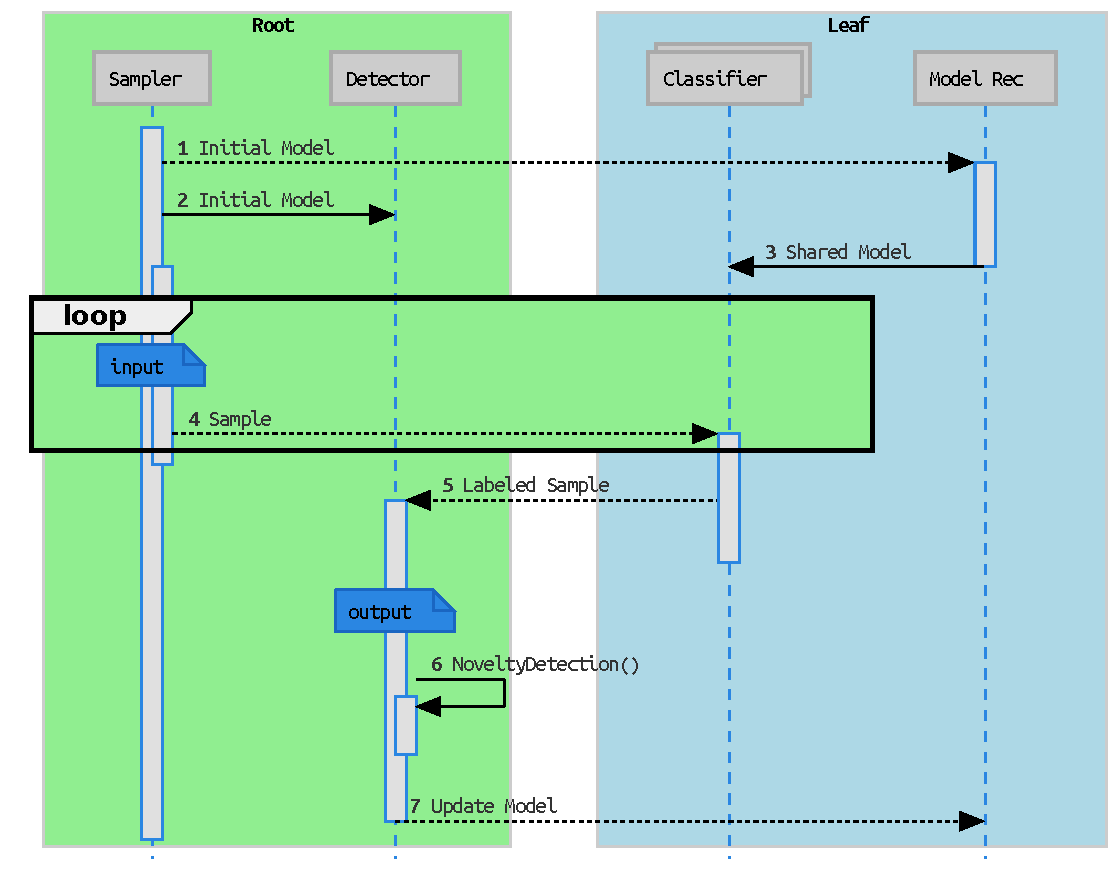
\includegraphics[width=\whencolumns{0.7\linewidth}{\columnwidth},page=1]{figures/lifecycle.uml.svg.pdf}
    \caption{\mfog life line overview.}
    \label{fig:mfog-mpi-life}
\end{figure}

\newlength{\intextsepBKP}
\setlength{\intextsepBKP}{\intextsep}
\setlength{\intextsep}{5pt}
% \newlength{\textfloatsepBKP}
% \setlength{\textfloatsepBKP}{\textfloatsep}
% \setlength{\textfloatsep}{5pt}
% \newlength{\floatsepBKP}
% \setlength{\floatsepBKP}{\floatsep}
% \setlength{\floatsep}{5pt}

\begin{algorithm}[h]
      \SetKwProg{Function}{Function}{:}{}
  \SetKwInOut{KwParams}{Parameters}
  \SetKwFor{With}{with}{}{}
  \SetKw{continue}{continue}
  \SetKw{break}{break}
  % 
  \SetKwData{mpiSize}{mpiSize}
  \SetKwData{mpiRank}{mpiRank}
  \SetKwData{EndOfStream}{EndOfStream}
  \SetKwData{noveltyDetectionTrigger}{noveltyDetectionTrigger}
  \SetKwData{cleaningWindow}{cleaningWindow}
  % 
  \SetKwFunction{Mfog}{Mfog}
  \SetKwFunction{Sampler}{Sampler}
  \SetKwFunction{Classifier}{Classifier}
  \SetKwFunction{Detector}{Detector}
  \SetKwFunction{modelReceiver}{modelReceiver}
  % 
  \SetKwFunction{typeOf}{typeOf}
  \SetKwFunction{Thread}{Thread}
  \SetKwFunction{Lock}{Lock}
  \SetKwFunction{readLock}{readLock}
  \SetKwFunction{writeLock}{writeLock}
  \SetKwFunction{receive}{receive}
  \SetKwFunction{send}{send}
  \SetKwFunction{broadcast}{broadcast}
  % 
  \SetKwFunction{nearestCluster}{nearestCluster}
  \SetKwFunction{NoveltyDetection}{NoveltyDetection}
  \SetKwFunction{handleModelSleep}{handleModelSleep}
  \SetKwFunction{removeOldSamples}{removeOldSamples}
  \SetKwFunction{now}{now}
  % 
    % 
    \SetKwInOut{KwParams}{Parameters}
    \KwParams{\mpiRank}
    \KwIn{inputStream}
    \KwOut{outputStream}
    \Function{\Mfog{inputStream, outputStream}}{
        Model $\leftarrow \emptyset$; ModelLock $\leftarrow$ \textbf{new} \Lock()\;
        \eIf(\emph{root}){\mpiRank $ = 0$}{
            \textbf{new} \Thread(\Detector, [outputStream, Model, ModelLock])\;
            \Sampler(inputStream, Model, ModelLock)\;
        }(\emph{leaf}){
            \textbf{new} \Thread(\modelReceiver, [Model, ModelLock])\;
            \Classifier(Model, ModelLock)\;
        }
    }
\caption{\mfog: main MPI entry-point.}
\label{alg:MFOG}
\end{algorithm}

\begin{algorithm}[h]
      \SetKwProg{Function}{Function}{:}{}
  \SetKwInOut{KwParams}{Parameters}
  \SetKwFor{With}{with}{}{}
  \SetKw{continue}{continue}
  \SetKw{break}{break}
  % 
  \SetKwData{mpiSize}{mpiSize}
  \SetKwData{mpiRank}{mpiRank}
  \SetKwData{EndOfStream}{EndOfStream}
  \SetKwData{noveltyDetectionTrigger}{noveltyDetectionTrigger}
  \SetKwData{cleaningWindow}{cleaningWindow}
  % 
  \SetKwFunction{Mfog}{Mfog}
  \SetKwFunction{Sampler}{Sampler}
  \SetKwFunction{Classifier}{Classifier}
  \SetKwFunction{Detector}{Detector}
  \SetKwFunction{modelReceiver}{modelReceiver}
  % 
  \SetKwFunction{typeOf}{typeOf}
  \SetKwFunction{Thread}{Thread}
  \SetKwFunction{Lock}{Lock}
  \SetKwFunction{readLock}{readLock}
  \SetKwFunction{writeLock}{writeLock}
  \SetKwFunction{receive}{receive}
  \SetKwFunction{send}{send}
  \SetKwFunction{broadcast}{broadcast}
  % 
  \SetKwFunction{nearestCluster}{nearestCluster}
  \SetKwFunction{NoveltyDetection}{NoveltyDetection}
  \SetKwFunction{handleModelSleep}{handleModelSleep}
  \SetKwFunction{removeOldSamples}{removeOldSamples}
  \SetKwFunction{now}{now}
  % 
    \Function{\Classifier{Model, ModelLock}}{
        \While{ True }{
            sampe $\leftarrow$ \receive(SampleType, root)\;
            \lIf{sample $=$ \EndOfStream}{\break}
            sample.label $\leftarrow$ ``unknown''\;
            \With{\readLock(ModelLock)}{
                nearest $\leftarrow$ \nearestCluster(sample, Model)\;
            }
            \If{nearest.distance $ \leq $ nearest.cluster.radius}{
                sample.label $\leftarrow$ nearest.cluster.label\;
            }
            \send(root, SampleType, sample)\;
        }
    }
    \Function{\modelReceiver{Model, ModelLock}}{
        \While{ True }{
            cl $\leftarrow$ \receive(ClusterType, root)\;
            \lIf{cl $=$ \EndOfStream}{\break}
            \With{writeLock(ModelLock)}{
                Model $\leftarrow$ Model $\cup$ cl\;
            }
        }
    }
  \caption{\mfog Leaf Tasks: Model Receiver and Classifier.}
  \label{alg:MFOG-leaf}
\end{algorithm}

\begin{algorithm}[t]
    \SetKwProg{Function}{Function}{:}{}
  \SetKwInOut{KwParams}{Parameters}
  \SetKwFor{With}{with}{}{}
  \SetKw{continue}{continue}
  \SetKw{break}{break}
  % 
  \SetKwData{mpiSize}{mpiSize}
  \SetKwData{mpiRank}{mpiRank}
  \SetKwData{EndOfStream}{EndOfStream}
  \SetKwData{noveltyDetectionTrigger}{noveltyDetectionTrigger}
  \SetKwData{cleaningWindow}{cleaningWindow}
  % 
  \SetKwFunction{Mfog}{Mfog}
  \SetKwFunction{Sampler}{Sampler}
  \SetKwFunction{Classifier}{Classifier}
  \SetKwFunction{Detector}{Detector}
  \SetKwFunction{modelReceiver}{modelReceiver}
  % 
  \SetKwFunction{typeOf}{typeOf}
  \SetKwFunction{Thread}{Thread}
  \SetKwFunction{Lock}{Lock}
  \SetKwFunction{readLock}{readLock}
  \SetKwFunction{writeLock}{writeLock}
  \SetKwFunction{receive}{receive}
  \SetKwFunction{send}{send}
  \SetKwFunction{broadcast}{broadcast}
  % 
  \SetKwFunction{nearestCluster}{nearestCluster}
  \SetKwFunction{NoveltyDetection}{NoveltyDetection}
  \SetKwFunction{handleModelSleep}{handleModelSleep}
  \SetKwFunction{removeOldSamples}{removeOldSamples}
  \SetKwFunction{now}{now}
  % 
  \KwParams{\mpiSize}
  \Function{\Sampler{inputStream, Model, ModelLock}}{
      dest $\leftarrow 1$\;
      \ForEach{sample $\in$ inputStream}{
          \If{\typeOf(sample) is Cluster}{
              \broadcast(ClusterType, sample, root)\;
              \With{\writeLock(ModelLock)}{
                  Model $\leftarrow$ Model $\cup$ sample\;
              }
              \continue\;
          }
          \send(dest, SampleType, sample)\;
          dest $\leftarrow$ dest $+ 1$\;
          \lIf{dest $>$ \mpiSize}{dest $\leftarrow$ 1}
      }
  }
  \KwParams{\cleaningWindow, \noveltyDetectionTrigger}
  \Function{\Detector{outputStream, Model, ModelLock}}{
        UnknownSet $\leftarrow \emptyset$; lastCleanup $\leftarrow 0$\;
        \While{ True }{
            sample $\leftarrow$ \receive(SampleType, any)\;
            \lIf{sample $=$ \EndOfStream}{\break}
            outputStream.append(sample)\;
            \If{sample.label $=$ ``unknown''}{
                UnknownSet $\leftarrow$ UnknownSet $\cup$ sample\;
                \If{$|\;UnknownSet\;| \geq$ \noveltyDetectionTrigger}{
                    novelties $\leftarrow$ \NoveltyDetection(Model, *UnknownSet)\;
                    \With{\writeLock(ModelLock)}{
                        Model $\leftarrow$ Model $\cup$ novelties\;
                    }
                    \ForEach{cluster $\in$ novelties}{
                        \broadcast(ClusterType, cluster, root)\;
                    }
                }
                \If{ sample.uid $ > $ ( lastCleanup $ + $ \cleaningWindow )}{
                    UnknownSet $\leftarrow$ \removeOldSamples(UnknownSet, lastCleanup)\;
                    lastCleanup $ \leftarrow $ sample.uid\;
                }
            }
        }
  }
\caption{\mfog Root Tasks: Sampler and Detector.}
\label{alg:MFOG-root}
\end{algorithm}

\setlength{\intextsep}{\intextsepBKP}
% \setlength{\textfloatsep}{\textfloatsepBKP}
% \setlength{\floatsep}{\floatsepBKP}
% \FloatBarrier
%\FloatBarrier

% ------------------------------------------------------------------------------
\section{Experiments and Results}
\label{sec:experiments}

For the experimental setup we dedicated three Raspberry Pi 3 model B single board computers
connected via Gigabit Ethernet Switch forming a simple cluster.
This cluster stored all source code, binaries (compiled and linked in place) and
datasets, being accessed via our laboratory network over Secure Shell (SSH).
All experiments were executed in this cluster for isolation of otherwise unforeseen
variations.

The dataset used is the December 2015 segment of
Kyoto 2006+ Dataset\footnote{Available at \url{http://www.takakura.com/Kyoto\_data/}}
(Traffic Data from Kyoto University's Honeypots)
\cite{Song2011}.
This segment was filtered (from $7\:865\:245$ instances) to only examples
associated to known attack types identified by existing IDS, and attack types
with more than $10\:000$ instances for significance as done by \cite{Cassales2019a}.
% , this removes 46,390 instances. TODO: revisar, pois 7M != 700K.
The remaining instantes then were transformed by normalization, transforming
each feature value space (e.g. IP Address, Duration, Service) to the
Real interval $[0, 1]$.
The result is stored in two sets, training set and test set, using the holdout
technique filtering in only normal class resulting in $72\:000$ instances for
training set and $653\:457$ for test set, containing $206\:278$ $N$ (normal) class
and $447\:179$ $A$ (attack) class.

% Count per class
%            id
% class        
% A      447179
% N      206278

% \begin{quote}
%   For the experiments, we used the Kyoto 2006+ dataset
%   which contains data collected from 2006 to December 2015.
%   We selected examples from one month, December, 2015. Only the examples of known
%   attack types and known IDS alert code with a minimum of 10,000 occurrences (for
%   significance) were considered. The offline training was performed with 72,000
%   examples (i.e., 10\% of the dataset) using the holdout technique.
%   \cite{Cassales2019a}
% \end{quote}

% \begin{highlight}
% O que quer testar com os experimentos.
% \begin{itemize}
%   \item Tese: Mostrar que detecção por novidade e classificação continua viável em fog.
%   \item Seria inviável por conta do atraso de distribuição de modelo e,
%   \item limitação pelo hardware pequeno.
%   \item MFOG: Um Agregador Regional, instalado na FOG, que observa a rede local.
% \end{itemize}

% Como realizou (cenário, rpi, setup, coleta de métricas).

% Quais resultados obteve.

% Como interpretar os resultados.
% \end{highlight}

% \hl{BEGIN Oritações de leitura das métricas e visualizações.}

\subsection{Metrics and Visualizations}

There are two broad evaluation metrics for each experiment:
a time mesure extracted by using \emph{GNU Time 1.9} and,
a set of qualitative mesures extracted by a python program.
The first metric is straightforward and is the time measure of the full program execution.
The latter metric is not as simple and for its extraction required a
purposely build python program.
This program takes two inputs, the test dataset and the captured output stream,
and outputs the confusion matrix, label-class association,
final quality summary with: Hits (accuracy), Misses (Err), Unknowns (UnkR); and
stream visualization chart with per example instance summary with novelty label markers.

For clarity, it is necessary to detail how to interpret and compare each metric,
as for some it is trivial but others are not so straightforward.

In the confusion matrix $M = m_{ij} \in \mathbb{N} ^{c \times{} l}$,
computed by our evaluation program,
each row denotes one of the datasets original (actual) class
and each column denotes the marked (predicted) label present in the captured output stream.
Thus, each cell $M_{c, l}$ contains the count of examples from the test dataset of class $c$
found in the output stream with the label $l$ assigned by the under evaluation experiment.
For the dataset under use, original classes are \emph{``N''} and \emph{``A''}, and
for the labels we have the training class \emph{``N''}, \emph{unknown} label \emph{``-''} and
the novelties $i \in \mathbb{N}$.

Added to the original confusion matrix $C$ are the rows \emph{Assigned} and
\emph{Hits}.
The former represents which original class $c$ (or if \emph{unknown}, \emph{``-''}) the
label $l$ is assigned to, this is computed by using the original class if
$c = l$ or by associated novelty label to original class as described in
\cite{DeFaria2015} section 4.1.
The latter row, \emph{Hits}, shows the true positive count for each label,
computed by coping the value of the cell $M_{c, l}$ where the label is the same
and the class $c$ is the value in the above \emph{Assigned} row.
The \emph{Hits} row is also used to compute the overall accuracy.
The complete matrix is shown in Tab. \ref{tab:java-matrix}.

% \begin{table*}[htb]\begin{center}
%   \caption{Reference implementation: Confusion Matrix and Qualitative Metrics}
%   \begin{tabular}{l|r|r|r|r|r|r|r|r|r|r|r|r|r|r}

Labels &     - &       N &    1 &    2 &    3 &  4 &   5 &    6 &    7 &     8 &    9 &    10 &   11 &  12 \\\hline
Classes  &       &         &      &      &      &    &     &      &      &       &      &       &      &     \\\hline
\hline
A        &  3774 &  438750 &  123 &  145 &  368 &  8 &  52 &  165 &    1 &  1046 &  161 &  2489 &   71 &  26 \\\hline
N        &  8206 &  193030 &    0 &   79 &   44 &  0 &   0 &    0 &  229 &   181 &  154 &  4066 &  289 &   0 \\\hline
\hline
Assigned &     - &       N &    A &    A &    A &  A &   A &    A &    N &     A &    A &     N &    N &   A \\\hline
Hits     &     0 &  193030 &  123 &  145 &  368 &  8 &  52 &  165 &  229 &  1046 &  161 &  4066 &  289 &  26 
\end{tabular}
% \begin{tabular}{l|r}

% Metric   &        Value \\\hline
% Metric   &              \\\hline
% \hline
% Hits     &     0.305618 \\\hline
% Misses   &     0.676049 \\\hline
% Unknowns &     0.018333 \\\hline
% Time     &  2761.830000 \\\hline
% System   &     7.150000 \\\hline
% Elapsed  &  2772.070000 
% \end{tabular}

%   \label{tab:java-matrix}
% \end{center}\end{table*}

\begin{table}[htb]
\begin{subtable}[h]{0.9\textwidth}\begin{center}
    \caption{Reference implementation}
    \begin{tabular}{l|r|r|r|r|r|r|r|r|r|r|r|r|r|r}

Labels &     - &       N &    1 &    2 &    3 &  4 &   5 &    6 &    7 &     8 &    9 &    10 &   11 &  12 \\\hline
Classes  &       &         &      &      &      &    &     &      &      &       &      &       &      &     \\\hline
\hline
A        &  3774 &  438750 &  123 &  145 &  368 &  8 &  52 &  165 &    1 &  1046 &  161 &  2489 &   71 &  26 \\\hline
N        &  8206 &  193030 &    0 &   79 &   44 &  0 &   0 &    0 &  229 &   181 &  154 &  4066 &  289 &   0 \\\hline
\hline
Assigned &     - &       N &    A &    A &    A &  A &   A &    A &    N &     A &    A &     N &    N &   A \\\hline
Hits     &     0 &  193030 &  123 &  145 &  368 &  8 &  52 &  165 &  229 &  1046 &  161 &  4066 &  289 &  26 
\end{tabular}
% \begin{tabular}{l|r}

% Metric   &        Value \\\hline
% Metric   &              \\\hline
% \hline
% Hits     &     0.305618 \\\hline
% Misses   &     0.676049 \\\hline
% Unknowns &     0.018333 \\\hline
% Time     &  2761.830000 \\\hline
% System   &     7.150000 \\\hline
% Elapsed  &  2772.070000 
% \end{tabular}

    \label{tab:java-matrix}
\end{center}\end{subtable}
\begin{subtable}[h]{0.9\textwidth}\begin{center}
    \caption{Serial implementation}
    \begin{tabular}{l|r|r|r|r|r|r|r|r|r|r|r}

Labels &      - &       N &   0 &    1 &    2 &   4 &   5 &  6 &   7 &   8 &  10 \\\hline
Classes  &        &         &     &      &      &     &     &    &     &     &     \\\hline
\hline
A        &  16086 &  429765 &  94 &  995 &  104 &   0 &  23 &  3 &  29 &  46 &  34 \\\hline
N        &  12481 &  193642 &   3 &   94 &    0 &  47 &   0 &  0 &   0 &  11 &   0 \\\hline
\hline
Assigned &      - &       N &   A &    A &    A &   N &   A &  A &   A &   A &   A \\\hline
Hits     &      0 &  193642 &  94 &  995 &  104 &  47 &  23 &  3 &  29 &  46 &  34 
\end{tabular}
% \begin{tabular}{l|r}

% Metric   &      Value \\\hline
% Metric   &            \\\hline
% \hline
% Hits     &   0.298438 \\\hline
% Misses   &   0.657843 \\\hline
% Unknowns &   0.043717 \\\hline
% Time     &  80.790000 \\\hline
% System   &  11.510000 \\\hline
% Elapsed  &  93.030000 
% \end{tabular}

    \label{tab:libc-matrix}
\end{center}\end{subtable}
\caption{Confusion Matrix and Qualitative Metrics}
\label{tab:confusion-matrixes}
\end{table}

For the metric summary table, six metrics from two sources are displayed.
Three metrics \emph{Hits} \emph{Unknowns} \emph{Misses} represented as ratio of the
captured output stream, extracted from the evaluation python
program, computed as follows:
\emph{Hits} (overall accuracy) is the summation of the homograph row in the
extended confusion matrix;
\emph{Unknowns} is the count of examples in the captured output stream marked
with the \emph{unknown} label \emph{``-''};
\emph{Misses} is the count of all examples in the captured output stream marked
with a label distinct from the \emph{Assigned} original class and are not marked
as unknown.
Lastly, \emph{Time}, \emph{System} and \emph{Elapsed} metrics represented in seconds,
are extracted from \emph{GNU Time}.
\emph{Time} is the amount of CPU seconds expended in user-mode
(indicates time used doing CPU intensive computing, e.g. math);
\emph{System} is the amount of CPU seconds expended in kernel-mode
(for our case it indicates time doing input or output);
\emph{Elapsed} is the real-world (wall clock) elapsed time
(indicates how long another system or person had to wait for the result).
To compare the time metric is simple, the lower time taken, the better.
Our four main experiments are shown in Tab. \ref{tab:exper-summary}.

Lastly, the stream visualization chart shows the summary quality metrics
(\emph{Hits} \emph{Unknowns} \emph{Misses})
computed for each example in the captured output stream.
This summary is computed for each example but it uses the \emph{Assigned} row
computed previously to evaluate \emph{Hits}, other metrics are derived as
described before.
Therefore, horizontal axis (x, domain) plots the index of the example and the
vertical axis (y, image) shows the metric computed until that example index on the captured
output stream.
Adding to the summary metrics, novelty label markers are represented as vertical
lines indicating \emph{when} in the captured output stream a new label first
appeared.
Some of the novelty label markers include the label itself ($l \in \mathbb{N}$)
for reference as if showing every label would turn this feature unreadable due
to overlapping.
Figure \ref{fig:validation-java-serial} shows two complete stream visualization charts.

\begin{figure*}[hbt]
  \centerline{
    \begin{subfigure}{.5\textwidth}
      \centering
      \includegraphics[width=\linewidth]{experiments/revised-java.log.png}
      \caption{Reference Implementation}
      \label{fig:validation-sub-java}
    \end{subfigure}
    \begin{subfigure}{.5\textwidth}
      \centering
      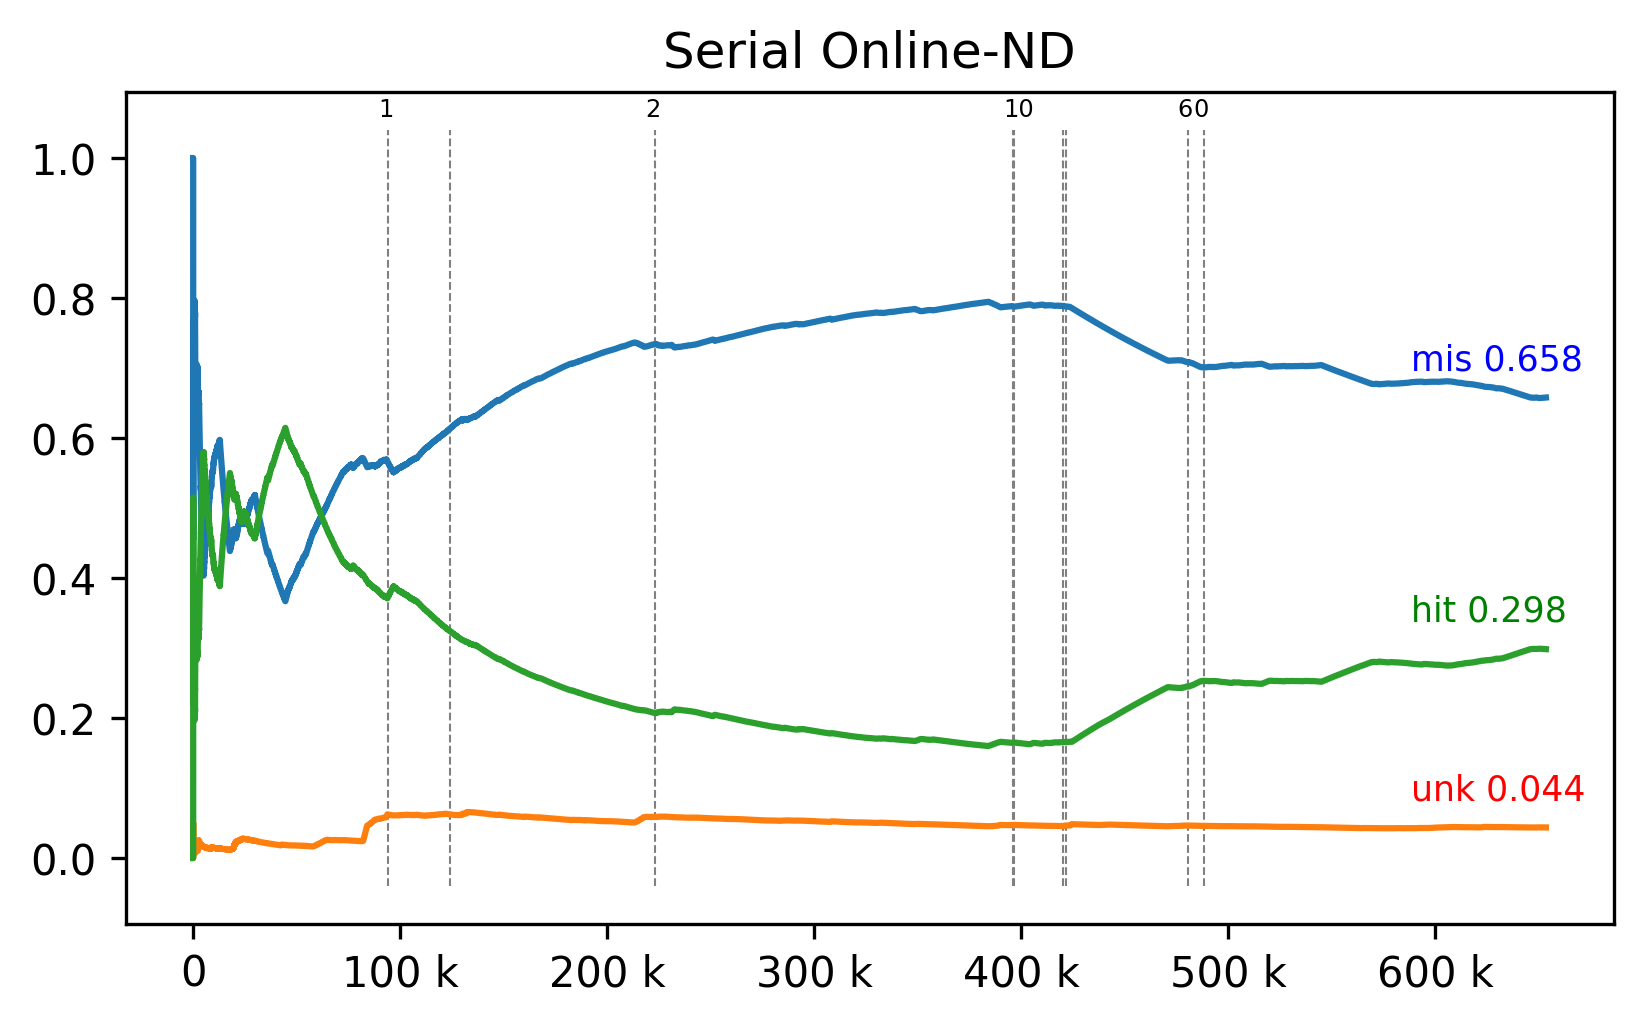
\includegraphics[width=\linewidth]{experiments/online-nd.log.png}
      \caption{Serial Implementation}
      \label{fig:validation-sub-serial}
    \end{subfigure}
  }
  \caption{Validation Comparison: Stream hits and novelties visualization}
  \label{fig:validation-java-serial}
\end{figure*}

% \hl{END Oritações de leitura das métricas e visualizações.}

\subsection{Results Discussion}

Four main experiments need detailed discussion:
(\emph{a}) reference implementation of Minas (\refminas) \cite{Faria2016minas};
(\emph{b}) new implementation in serial mode;
(\emph{c}) new implementation in single-node, multi-task mode and
(\emph{d}) new implementation in multi-node, multi-task mode.
Each experiment uses the adequate binary executable, initial model
(or training set for the reference implementation) and test set
to compute a resulting output stream which is stored for qualitative evaluation.
The summary of all four experiments is shown in Table \ref{tab:exper-summary}.

\begin{table}[hbt]\begin{center}
  \caption{Collected Metrics Summary. \color{red}{deixo os tempos com ou sem a soma do tempo offline?}}
  % \begin{tabular}{l|r|r|r|r}
%          &    Exp. (a)  & Exp. (b)   & Exp. (c)    & Exp. (d)   \\\hline
% Hits     &     0.305618 &   0.298438 &    0.312416 &    0.312478    \\\hline
% Misses   &     0.676049 &   0.657843 &    0.664061 &    0.663802    \\\hline
% Unknowns &     0.018333 &   0.043717 &    0.023521 &    0.023718    \\\hline
% Time     &  2761.830000 &  80.790000 &  522.100000 &  207.140000    \\\hline
% System   &     7.150000 &  11.510000 &   47.770000 &  157.610000    \\\hline
% Elapsed  &  2772.070000 &  93.030000 &  145.040000 &   95.380000    
% \end{tabular}

% java -ea -classpath bin/minas/revised.jar: NoveltyDetection.MinasRevised datasets/training.csv datasets/test.csv out/revised-java.log true
% 	2761.82 user	7.15 system	46:12.07 elapsed

% ./bin/offline
% 	193.94 user	0.05 system	3:14.04 elapsed

% "./bin/ond
% 	80.79 user	11.51 system	1:33.02 elapsed

% mpirun -n 12 -hostfile ./conf/hostsfile ./bin/tmpi
% 	207.13 user	157.61 system	1:35.38 elapsed

\newcommand{\mr}[1]{\multirow{2}{*}{#1}}

\begin{tabular}{l|r|r|r|r|r}
                & \refminas (a)  & Offline       & Serial (b)      & Single Node (c) & Multi Node (d)  \\\hline
\mr{Hits}       & $\ 199708\ $   &               & $\ 195017\ $    & $\ 204151\ $    & $\ 204191\ $    \\
                & $\ 0.305618\ $ &               & $\ 0.298438\ $  & $\ 0.312416\ $  & $\ 0.312478\ $  \\
\hline
\mr{Misses}     & $\ 441769\ $   &               & $\ 429873\ $    & $\ 433936\ $    & $\ 433767\ $    \\
                & $\ 0.676049\ $ &               & $\ 0.657843\ $  & $\ 0.664061\ $  & $\ 0.663802\ $  \\
\hline
\mr{Unknowns}   & $\ 11980\ $    &               & $\ 28567\ $     & $\ 15370\ $     & $\ 15499\ $     \\
                & $\ 0.018333\ $ &               & $\ 0.043717\ $  & $\ 0.023521\ $  & $\ 0.023718\ $  \\
\hline
Time            & $\ 2761.83\ $  & $\ 194.12\ $  & $\ 80.79000\ $  & $\ 522.1000\ $  & $\ 207.1400\ $  \\\hline
System          & $\ 7.15\ $     & $\  0.075\ $  & $\ 11.51000\ $  & $\  47.7700\ $  & $\ 157.6100\ $  \\\hline
Elapsed         & $\ 2772.07\ $  & $\ 194.27\ $  & $\ 93.03000\ $  & $\ 145.0400\ $  & $\  95.3800\ $  
\end{tabular}


  \label{tab:exper-summary}
\end{center}\end{table}

The first two experiments (\emph{a} and \emph{b}) comparison does serve as
validation for our implementation, while the latter three (\emph{b}, \emph{c}
and \emph{d}) serves as showcase for the effects of distribution.

As stated, to validate our implementation we compare it to \refminas
(the original \minas companion implementation), so we extracted the same metrics
using same process for both \emph{a} and \emph{b}, they can be viewed on
Tables \ref{tab:java-matrix}, \ref{tab:libc-matrix} and for ease of comparison
on Table \ref{tab:exper-summary} the summary can be compared side by side.

In general the observed classification quality metrics are very similar,
they diverge slightly where \emph{a} has more \emph{Hits} and \emph{Misses}
whereas \emph{b} shifted those to \emph{Unknowns}.
This phenomenon was watched very closely during development and we found that
small changes to MINAS parameters, MINAS internals like K-means ordering,
cluster edge inclusion and cluster radius formula as stated in
Subsection \ref{sec:implementation}.
As for the efficiency metrics on Table \ref{tab:exper-summary}
our implementation used less time to analyze the test data set,
this is due to small optimizations on the minimal sample to cluster center
on the classifier task and more importantly on the stop condition
on the internal K-means algorithm, while \refminas uses a fixed iteration
limit of $100$, our implementations adds the ``no improvment'' check
and thus stops earlier on most cases and this in turn reduces time taken
on the Novelty Detection step.
Also note that \refminas time includes the Offline phase while
our implementation runs it once and reuses the initial model for
\emph{b}, \emph{c} and \emph{d}.

As for the effects of running a MPI cluster with our implementation
we observe an increase of time when e go from 
\st{we have to say it is pretty shitty because of our choice of distribution 
using round-robin, use some load balancing and micro-batching for better results.}
Nevertheless, we can also show the effects of delay in the
Classify, Novelty Detect, Model Update and Classify loop, as in the
first non-serial experiment \emph{b} we observe a reduction in Novelty Labels
on the Confusion Matrix (Tables \ref{tab:libc-matrix} and \ref{tab:single-node-matrix})
from $10$ to $4$.
The same effect is observed on the stream visualization as well, where
Figure \ref{fig:validation-sub-serial}

% \todo{discutir o delay de 80k entre etiqueta 0 em serial vs node}

When observing the stream visualization on figure \ref{fig:cluster-sub-multi}

\begin{table}[htb]
\begin{subtable}[h]{0.9\textwidth}\begin{center}
    \caption{Parallel single-node}
    \begin{tabular}{l|r|r|r|r|r|r|r}

Labels &      - &       N &    0 &    1 &   2 &  3 &  4 \\\hline
Classes  &        &         &      &      &     &    &    \\\hline
\hline
A        &  12282 &  433797 &  147 &  952 &   0 &  0 &  1 \\\hline
N        &   3088 &  203019 &   40 &   99 &  27 &  5 &  0 \\\hline
\hline
Assigned &      - &       N &    A &    A &   N &  N &  A \\\hline
Hits     &      0 &  203019 &  147 &  952 &  27 &  5 &  1 
\end{tabular}
% \begin{tabular}{l|r}

% Metric   &       Value \\\hline
% \hline
% Hits     &    0.312416 \\\hline
% Misses   &    0.664061 \\\hline
% Unknowns &    0.023521 \\\hline
% Time     &  522.100000 \\\hline
% System   &   47.770000 \\\hline
% Elapsed  &  145.040000 
% \end{tabular}

    \label{tab:single-node-matrix}
\end{center}\end{subtable}
\begin{subtable}[h]{0.9\textwidth}\begin{center}
    \caption{Parallel multi-node}
    \begin{tabular}{l|r|r|r|r|r|r|r}

Labels &      - &       N &    0 &    1 &    2 &    3 &  4 \\\hline
Classes  &        &         &      &      &      &      &    \\\hline
\hline
A        &  12378 &  433631 &  117 &  886 &    0 &  162 &  5 \\\hline
N        &   3121 &  202916 &   40 &   96 &  105 &    0 &  0 \\\hline
\hline
Assigned &      - &       N &    A &    A &    N &    A &  A \\\hline
Hits     &      0 &  202916 &  117 &  886 &  105 &  162 &  5 
\end{tabular}
% \begin{tabular}{l|r}

% Metric   &       Value \\\hline
% \hline
% Hits     &    0.312478 \\\hline
% Misses   &    0.663802 \\\hline
% Unknowns &    0.023718 \\\hline
% Time     &  207.140000 \\\hline
% System   &  157.610000 \\\hline
% Elapsed  &   95.380000 
% \end{tabular}

    \label{tab:multi-node-matrix}
\end{center}\end{subtable}
\caption{Confusion Matrix and Qualitative Metrics for MPI Clusters.}
\label{tab:confusion-matrixes}
\end{table}

% 22.40 user	0.02 system	0:22.48 elapsed

% \begin{table*}[htb]\begin{center}
%   \caption{Serial implementation: Confusion Matrix and Qualitative Metrics}
%   \begin{tabular}{l|r|r|r|r|r|r|r|r|r|r|r}

Labels &      - &       N &   0 &    1 &    2 &   4 &   5 &  6 &   7 &   8 &  10 \\\hline
Classes  &        &         &     &      &      &     &     &    &     &     &     \\\hline
\hline
A        &  16086 &  429765 &  94 &  995 &  104 &   0 &  23 &  3 &  29 &  46 &  34 \\\hline
N        &  12481 &  193642 &   3 &   94 &    0 &  47 &   0 &  0 &   0 &  11 &   0 \\\hline
\hline
Assigned &      - &       N &   A &    A &    A &   N &   A &  A &   A &   A &   A \\\hline
Hits     &      0 &  193642 &  94 &  995 &  104 &  47 &  23 &  3 &  29 &  46 &  34 
\end{tabular}
% \begin{tabular}{l|r}

% Metric   &      Value \\\hline
% Metric   &            \\\hline
% \hline
% Hits     &   0.298438 \\\hline
% Misses   &   0.657843 \\\hline
% Unknowns &   0.043717 \\\hline
% Time     &  80.790000 \\\hline
% System   &  11.510000 \\\hline
% Elapsed  &  93.030000 
% \end{tabular}

%   \label{tab:libc-matrix}
% \end{center}\end{table*}

\begin{figure*}[htb]
  \centerline{
    \begin{subfigure}{.5\textwidth}
      \centering
      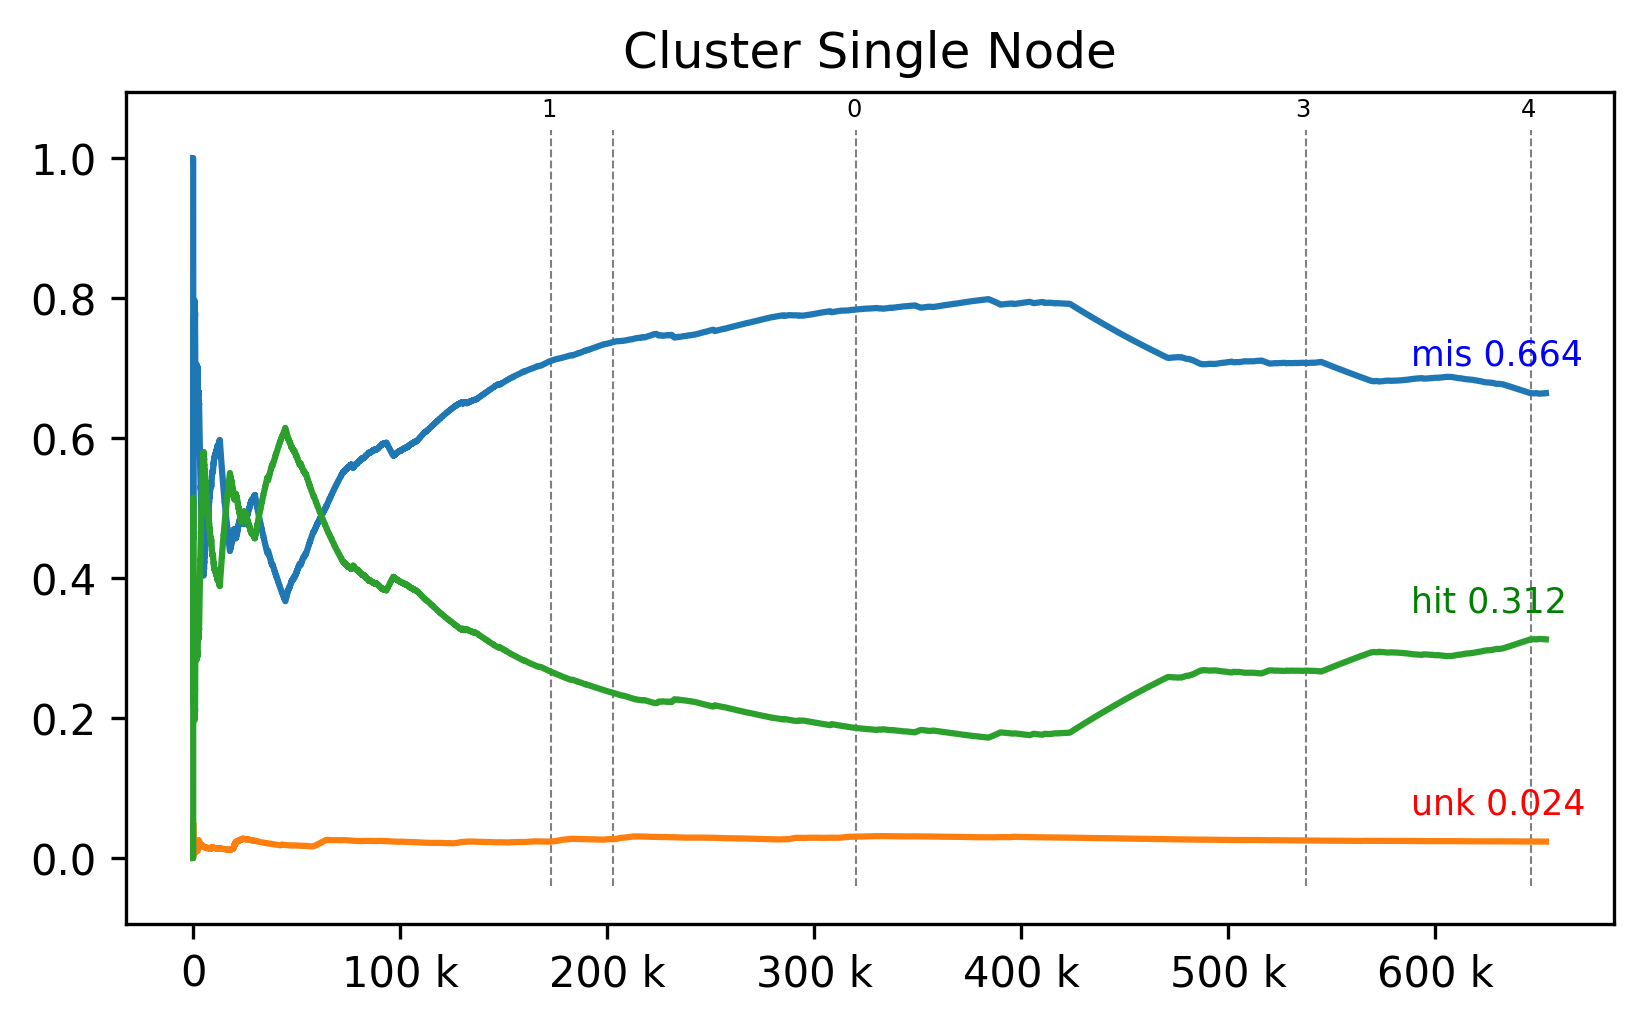
\includegraphics[width=\linewidth]{experiments/tmi-base.log.png}
      \caption{Parallel single-node}
      \label{fig:cluster-sub-single}
    \end{subfigure}
    \begin{subfigure}{.5\textwidth}
      \centering
      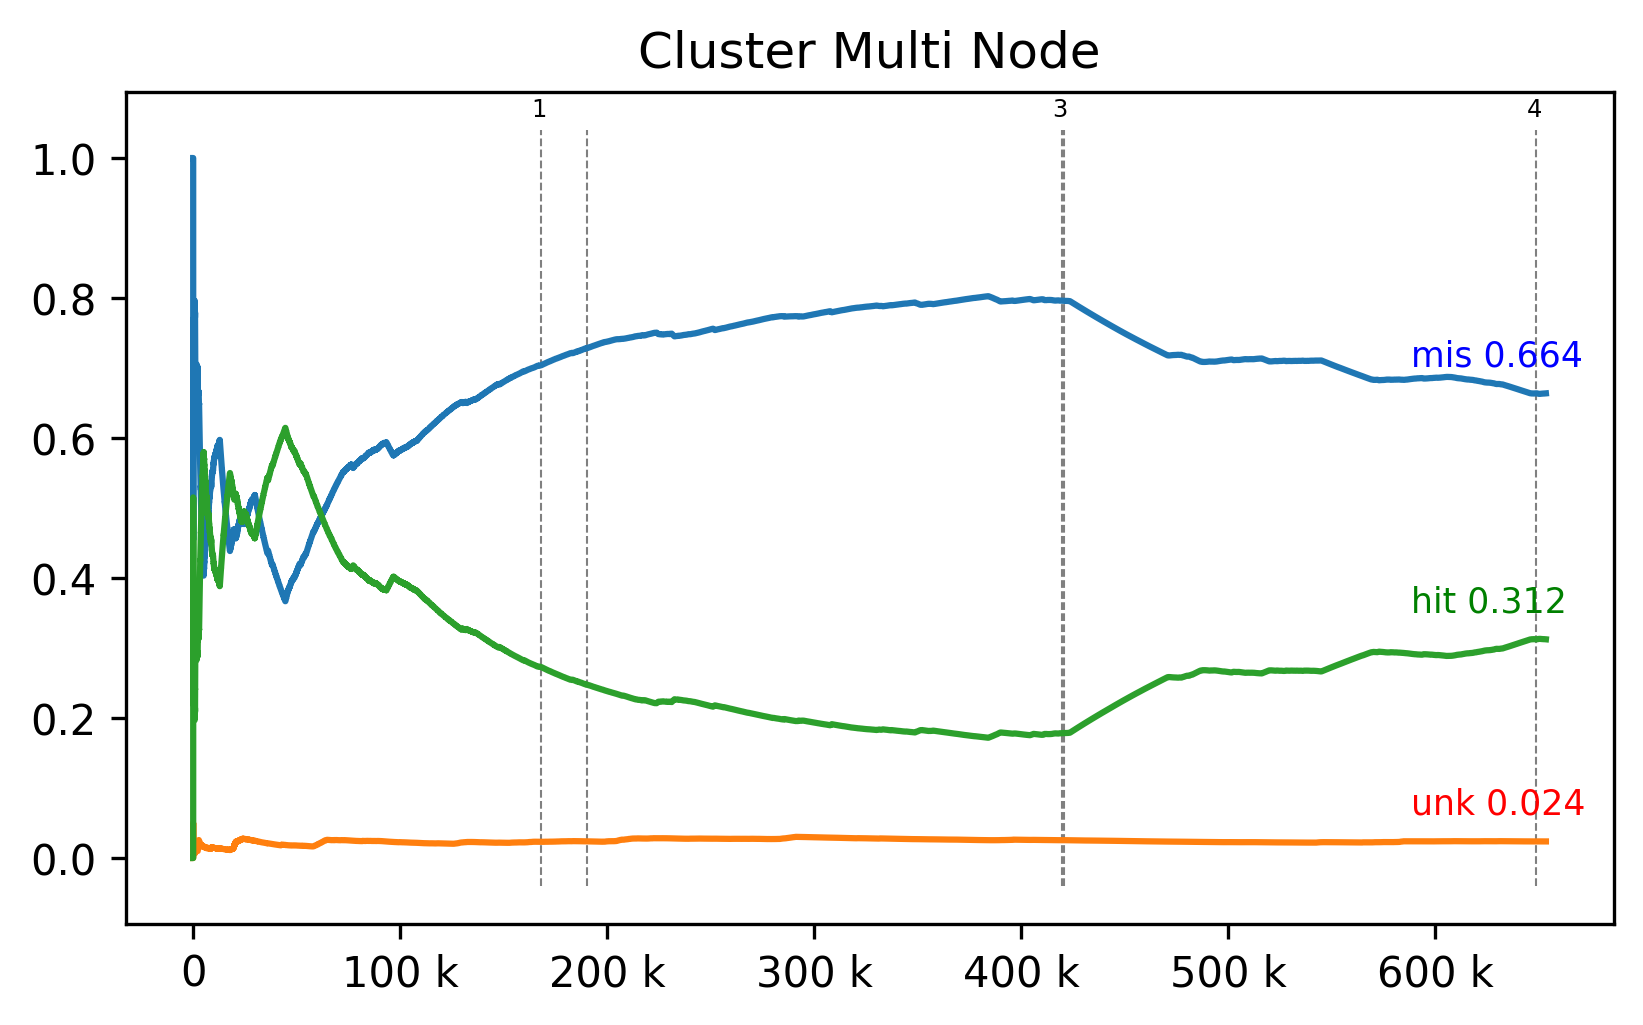
\includegraphics[width=\linewidth]{experiments/tmi-n12.log.png}
      \caption{Parallel multi-node}
      \label{fig:cluster-sub-multi}
    \end{subfigure}
    % \begin{subfigure}{.5\textwidth}
    %   \centering
    %   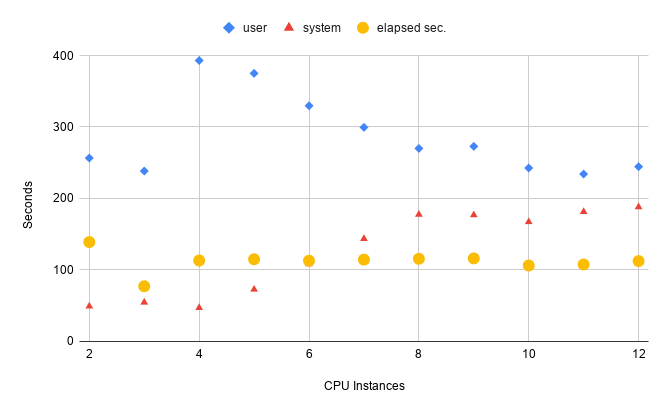
\includegraphics[width=\linewidth]{experiments/speedup-clean.png}
    %   \caption{Time measurements per added instance}
    %   \label{fig:cluster-sub-multi}
    % \end{subfigure}
  }
  \caption{Parallelism Comparison: Stream hits and novelties visualization}
  \label{fig:cluster}
\end{figure*}

\begin{figure}
  \centering
  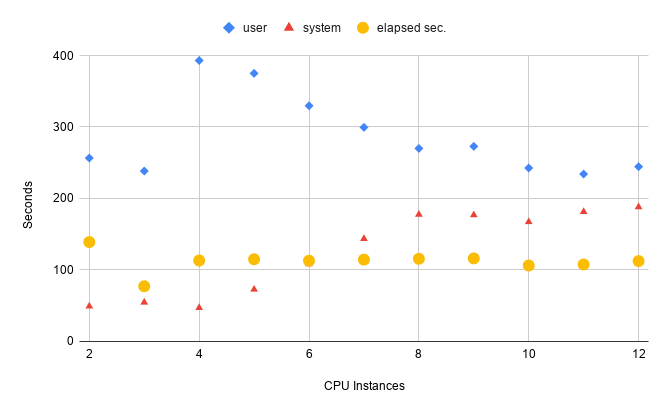
\includegraphics[width=\linewidth]{experiments/speedup-clean.png}
  \caption{Time measurements per added instance}
  \label{fig:speedup}
\end{figure}

% \begin{table}[htb]\begin{center}
%   \caption{Parallel single-node: Confusion Matrix and Qualitative Metrics}
%   \begin{tabular}{l|r|r|r|r|r|r|r}

Labels &      - &       N &    0 &    1 &   2 &  3 &  4 \\\hline
Classes  &        &         &      &      &     &    &    \\\hline
\hline
A        &  12282 &  433797 &  147 &  952 &   0 &  0 &  1 \\\hline
N        &   3088 &  203019 &   40 &   99 &  27 &  5 &  0 \\\hline
\hline
Assigned &      - &       N &    A &    A &   N &  N &  A \\\hline
Hits     &      0 &  203019 &  147 &  952 &  27 &  5 &  1 
\end{tabular}
% \begin{tabular}{l|r}

% Metric   &       Value \\\hline
% \hline
% Hits     &    0.312416 \\\hline
% Misses   &    0.664061 \\\hline
% Unknowns &    0.023521 \\\hline
% Time     &  522.100000 \\\hline
% System   &   47.770000 \\\hline
% Elapsed  &  145.040000 
% \end{tabular}

%   \label{tab:single-node-matrix}
% \end{center}\end{table}

% \setcounter{MaxMatrixCols}{20}
% \begin{table*}[htb]
  %   \begin{center}
    %     \caption{Reference implementation: Confusion Matrix and Qualitative Metrics}
    %     \begin{math}\begin{pmatrix}
      %       - & N & 1 & 2 & 3 & 4 & 5 & 6 & 7 & 8 & 9 & 10 & 11 & 12
%     \end{pmatrix}\end{math}
%     \begin{math}\begin{pmatrix}
%     3774 &  438750 &  123 &  145 &  368 &  8 &  52 &  165 &    1 &  1046 &  161 &  2489 &   71 &  26 \\
%     8206 &  193030 &    0 &   79 &   44 &  0 &   0 &    0 &  229 &   181 &  154 &  4066 &  289 &   0
%     \end{pmatrix}\end{math}
%     \begin{math}\begin{pmatrix}
%       - &       N &    A &    A &    A &  A &   A &    A &    N &     A &    A &     N &    N &   A \\
%       0 &  193030 &  123 &  145 &  368 &  8 &  52 &  165 &  229 &  1046 &  161 &  4066 &  289 &  26 
%     \end{pmatrix}\end{math}
%     \label{math-tab}
%   \end{center}
% \end{table*}

% \begin{figure*}
%   \centering
%   \centerline{
%     \includegraphics[width=0.45\textwidth]{../experiments/revised-java.log.png}
%     \includegraphics[width=0.45\textwidth]{../experiments/revised-java.log.png}
%   }
%   \\
%   \centerline{
%     \includegraphics[width=0.45\textwidth]{../experiments/revised-java.log.png}
%     \includegraphics[width=0.45\textwidth]{../experiments/revised-java.log.png}
%   }
% \label{fig1} 
% \end{figure*}

% \begin{highlight}

% \end{highlight}

%\FloatBarrier

% ----------------------------------------------------------------------------------------------------------------------
\section{Conclusion} 
\label{sec:conclusion}

% Conexão entre Intro e Conclusão
% - Novelty Detection in Data Streams já é validado
% - IoT leva a ambientes Edge com nós pequenos
% - Nesse ambiente propomos \mfog
%     - Modelamos o software, implementamos
% - Testamos e observamos tempo e qualidade
%     - Tempo adequado mas sub-linear, pouco efeito na qualidade
% - Melhres distribuiçõpes são possíveis
%     - mais roots (melhor algo de distribuição)
%     - mini batching

Data Stream Novelty Detection (\nd) can be a useful mechanism for Network
Intrusion Detection (\nids) in IoT environments. It can also serve other related applications of \nd using continuous
network or system behavior monitoring and analysis.
% However, in the \iot context, it is expected that small edge devices perform
% such maintenance tasks.
Regarding the tremendous amount of data that must be processed in the flow analysis for \nd, it 
is relevant that this processing takes place at the edge of the network. 
However, one relevant shortcoming of the IoT, in this case, is the reduced processing capacity of such edge devices. 

In this sense, we have put together and evaluated a distributed architecture for
performing \nd applied at network flow descriptors at the edge.
% In that small computing on edge scenario, w
Our proposal, \mfog, is a distributed \nd implementation based on the \minas
algorithm and the main goal of this work is to observe the effects of our
approach to a previously sequential only algorithm, especially in regards to
time and quality metrics.

% \mfog is a demonstration piece

% pode ser a conclusão do abstract
While there is some impact on the predictive metrics, this is not reflected on
overall classification quality metrics indicating that distribution of \minas
has a negligible loss of accuracy.
% but is overshadow by the benefits of scalability.
In regards to time and scale, our distributed executions was faster than the 
previous sequential implementation of \minas, but efficient data distribution was not achieved as the
observed time with each added node remained near constant.
% In our experiments, a months worth of traffic flow descriptors is processed in
% around $300$ seconds even with non-optimal load sharing round-robin strategy.
% (single sample round-robin that incurs the bigger networking overhead),
% sparing use of memory (unknown buffer limited to a fraction of the available memory),
% and potential system slowdown due to cascading effects on networking queue
% (caused by the Detector Module when its unknown buffer is full and novelty
% detection task is under way as it still a non-stream oriented algorithm limited
% to a single batch of fixed memory).

% Acho que trocaria a úlitma frase por algo mais conclusivo para fechar o artigo
Overall, \mfog and the idea of using distributed flow classification and novelty
detection while minimizing memory usage to fit in smaller devices at the edge of
the network is a viable and promising solution.
Further work includes the investigation of other \nd algorithms, other clustering
algorithms in \minas and analysis of varying load balancing strategies.
% also considering using a distributed version of the k-means clustering.

% Our treatment involved reworking the algorithm and implementation to be
% distributed and %to minimize the memory usage as 
% minimizing memory usage to fit in smaller devices.
% Other algorithms still need a similar treatment and, more importantly, other
% distribution strategies should be considered.

% Aplicação em cenário real.

% ----------------------------------------------------------------------------------------------------------------------
\section*{Acknowledgment}

% The preferred spelling of the word ``acknowledgment'' in America is without an ``e'' after the ``g''.
% Avoid the stilted expression ``one of us (R. B. G.) thanks $\ldots$''.
% Instead, try ``R. B. G. thanks$\ldots$''.
% Put sponsor  acknowledgments in the unnumbered footnote on the first page.
This study was financed in part by the Coordenação de Aperfeiçoamento de Pessoal de
Nível Superior - Brasil (CAPES) - Finance Code 001,
and Programa Institucional de Internacionalização – CAPES-PrInt UFSCar (Contract 88887.373234/2019-00). 
Authors also thank Stic AMSUD (project 20-STIC-09), FAPESP (contract numbers  2018/22979-2, and 2015/24461-2) and CNPq (Contract 167345/2018-4) for their support.


\bibliographystyle{lib/splncs04.bst}
\bibliography{99-refs-ISCC}
\end{document}
